\chapter{IP routing}
\label{chap:ip-routing}

It's time now to turn our focus toward the core topic of the ubiquitous IP routing process.
It's integral to networking because it pertains to all routers and configurations that use it, which is easily the lion's share.
IP routing is basically the process of moving packets from one network to another network using routers.
%And by routers, I mean Cisco routers, of course!
However, the terms \emph{router} and \emph{layer 3 device} are interchangeable, and throughout this chapter when I use the term \emph{router},
I am referring to any layer 3 device.

Before jumping into this chapter, I want to make sure you understand the difference between a \emph{routing protocol} and a \emph{routed protocol}.
Routers use routing protocols to dynamically find all networks within the greater internetwork and to ensure that all routers have the same routing table.
Routing protocols are also employed to determine the best path a packet should take through an internetwork t get to its destination most efficiently.
RIP, RIPv2, EIGRP, and OSPF are great examples of the most common routing protocols.

Once all routers know about all networks, a routed protocol can be used to send user data (packets) through the established enterprise.
Routed protocols are assigned to an interface and determine the method of packet delivery.
Examples of routed protocols are IPv4 and IPv6.

I'm pretty confident I don't have to underscore how crucial it is for you to have this chapter's material down to a near instinctive level.
IP routing is innately what routers do, and they do it very well,
so having a firm grasp of the fundamentals and basics of this topic is vital if you want to excel during the exam and in a real-world networking environment as well!

In this chapter, I'm going to show you how to configure and verify IP routing with Cisco routers and guide you through these five key subjects:
\begin{itemize}
\item routing basics
\item the IP routing process
\item static routing
\item default routing
\item dynamic routing
\end{itemize}

I want to start by nailing down the basics of how packets actually move through an internetwork, so let's get started!



\section{Routing basics}

Once you create an internetwork by connecting your WANs and LANs to a
router, you'll need to configure logical network addresses, like IP
addresses, to all hosts on that internetwork for them to communicate
successfully throughout it.

The term \emph{routing} refers to taking a packet from one device and
sending it through the network to another device on a different network.
Routers don't really care about hosts---they only care about networks
and the best path to each one of them. The logical network address of
the destination host is key to getting packets through a routed network.
It's the hardware address of the host that's used to deliver the packet
from a router and ensure it arrives at the correct destination host.

Routing is irrelevant if your network has no routers because their job
is to route traffic to all the networks in your internetwork, but this
is rarely the case! So here's an important list of the minimum factors a
router must know to be able to effectively route packets:

\begin{itemize}
\item destination address
\item neighbor routers from which it can learn about remote networks
\item possible routes to all remote networks
\item the best route to each remote network
\item how to maintain and verify routing information
\end{itemize}

The router learns about remote networks from neighboring routers or from
an administrator. The router then builds a routing table, which is
basically a map of the internetwork, and it describes how to find remote
networks. If a network is directly connected, then the router already
knows how to get to it.

But if a network isn't directly connected to the router, the router must
use one of two ways to learn how to get to the remote network. The
\emph{static routing} method requires someone to hand-type all network
locations into the routing table, which can be a pretty daunting task
when used on all but the smallest of networks!

Conversely, when \emph{dynamic routing} is used, a protocol on one
router communicates with the same protocol running on neighboring
routers. The routers then update each other about all the networks they
know about and place this information into the routing table. If a
change occurs in the network, the dynamic routing protocols
automatically inform all routers about the event. If static routing is
used, the administrator is responsible for updating all changes by hand
onto all routers. Most people usually use a combination of dynamic and
static routing to administer a large network.

Before we jump into the IP routing process, let's take a look at a very
simple example that demonstrates how a router uses the routing table to
route packets out of an interface. We'll be going into a more detailed
study of the process soon, but I want to show you something called the
``longest match rule'' first. With it, IP will scan a routing table to
find the longest match as compared to the destination address of a packet.
Let's take a look at \cref{fig:simple-routing-example} to get a picture of this process.


\begin{figure}
   \centering
   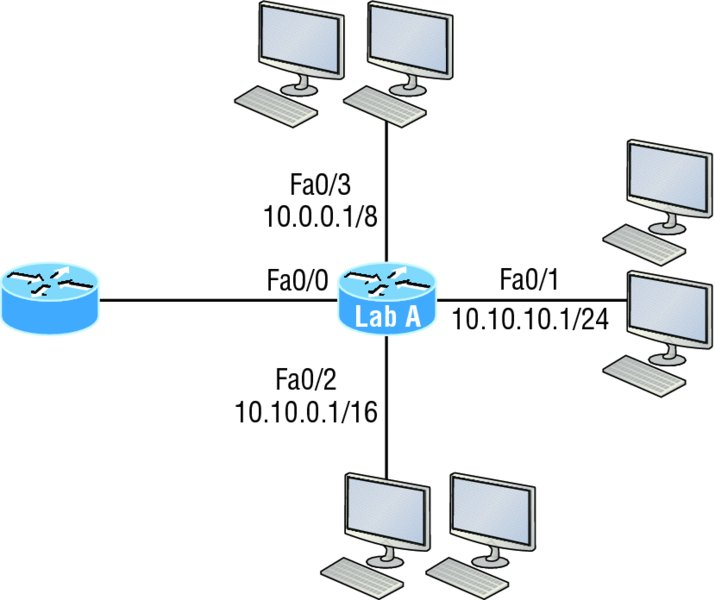
\includegraphics[width=.5\textwidth]{images/c09f001.jpg}
   \caption{A simple routing example}
   \label{fig:simple-routing-example}
\end{figure}


\Cref{fig:simple-routing-example} shows a simple network.
Lab\_A has four interfaces.
Can you see which interface will be used to forward an IP datagram to a host with a destination IP address of 10.10.10.30?

By using the command \texttt{show\ ip\ route} on a router, we can see
the routing table (map of the internetwork) that Lab\_A has used to make
its forwarding decisions:

\begin{verbatim}
Lab_A#sh ip route
Codes: L - local, C - connected, S - static,
[output cut]
        10.0.0.0/8 is variably subnetted, 6 subnets, 4 masks
C       10.0.0.0/8 is directly connected, FastEthernet0/3
L       10.0.0.1/32 is directly connected, FastEthernet0/3
C       10.10.0.0/16 is directly connected, FastEthernet0/2
L       10.10.0.1/32 is directly connected, FastEthernet0/2
C       10.10.10.0/24 is directly connected, FastEthernet0/1
L       10.10.10.1/32 is directly connected, FastEthernet0/1
S*      0.0.0.0/0 is directly connected, FastEthernet0/0
\end{verbatim}

The \texttt{C} in the routing table output means that the networks
listed are ``directly connected,'' and until we add a routing protocol
like RIPv2, OSPF, etc. to the routers in our internetwork, or enter
static routes, only directly connected networks will show up in our
routing table. But wait---what about that \texttt{L} in the routing
table---that's new, isn't it? Yes it is, because in the new Cisco IOS 15
code, Cisco defines a different route, called a local host route. Each
local route has a /32 prefix, defining a route just for the one address.
So in this example, the router has relied upon these routes that list
their own local IP addresses to more efficiently forward packets to the
router itself.

\protect\hypertarget{c09.xhtmlux5cux23Page_361}{}{}So let's get back to
the original question: By looking at the figure and the output of the
routing table, can you determine what IP will do with a received packet
that has a destination IP address of 10.10.10.30? The answer is that the
router will packet-switch the packet to interface FastEthernet 0/1,
which will frame the packet and then send it out on the network segment.
This is referred to as frame rewrite. Based upon the longest match rule,
IP would look for 10.10.10.30, and if that isn't found in the table,
then IP would search for 10.10.10.0, then 10.10.0.0, and so on until a
route is discovered.

Here's another example: Based on the output of the next routing table,
which interface will a packet with a destination address of 10.10.10.14
be forwarded from?

\begin{verbatim}
Lab_A#sh ip route
[output cut]
Gateway of last resort is not set
C      10.10.10.16/28 is directly connected, FastEthernet0/0
L      10.10.10.17/32 is directly connected, FastEthernet0/0
C      10.10.10.8/29 is directly connected, FastEthernet0/1
L      10.10.10.9/32 is directly connected, FastEthernet0/1
C      10.10.10.4/30 is directly connected, FastEthernet0/2
L      10.10.10.5/32 is directly connected, FastEthernet0/2
C      10.10.10.0/30 is directly connected, Serial 0/0
L      10.10.10.1/32 is directly connected, Serial0/0
\end{verbatim}

To figure this out, look closely at the output until you see that the
network is subnetted and each interface has a different mask. And I have
to tell you---you just can't answer this question if you can't subnet!
10.10.10.14 would be a host in the 10.10.10.8/29 subnet that's connected
to the FastEthernet0/1 interface. Don't freak if you're struggling and
don't get this! Instead, just go back and reread Chapter 4, ``Easy
Subnetting,'' until it becomes clear to you.

\section{The IP Routing Process}

The IP routing process is fairly simple and doesn't change, regardless
of the size of your network. For a good example of this fact, I'll use
\protect\hyperlink{c09.xhtmlux5cux23figure9-2}{Figure 9.2} to describe
step-by-step what happens when Host A wants to communicate with Host B
on a different network.

\begin{figure}
\centering
%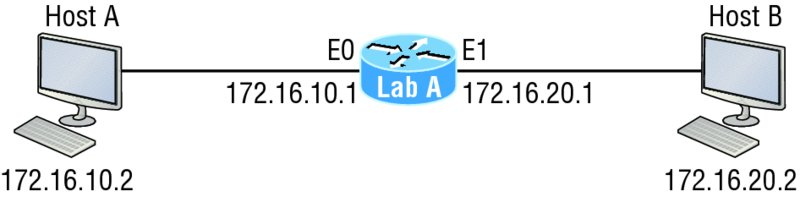
\includegraphics{images/c09f002.jpg}
\caption{{\protect\hyperlink{c09.xhtmlux5cux23figureanchor9-2}{\textbf{FIGURE
9.2}} IP routing example using two hosts and one router}}
\end{figure}

\protect\hypertarget{c09.xhtmlux5cux23Page_362}{}{}In
\protect\hyperlink{c09.xhtmlux5cux23figure9-2}{Figure 9.2} a user on
Host\_A pinged Host\_B's IP address. Routing doesn't get any simpler
than this, but it still involves a lot of steps, so let's work through
them now:

\begin{enumerate}
\item
  Internet Control Message Protocol (ICMP) creates an echo request
  payload, which is simply the alphabet in the data field.
\item
  ICMP hands that payload to Internet Protocol (IP), which then creates
  a packet. At a minimum, this packet contains an IP source address, an
  IP destination address, and a Protocol field with 01h. Don't forget
  that Cisco likes to use \emph{0x} in front of hex characters, so this
  could also look like 0x01. This tells the receiving host to whom it
  should hand the payload when the destination is reached---in this
  example, ICMP.
\item
  Once the packet is created, IP determines whether the destination IP
  address is on the local network or a remote one.
\item
  Since IP has determined that this is a remote request, the packet must
  be sent to the default gateway so it can be routed to the remote
  network. The Registry in Windows is parsed to find the configured
  default gateway.
\item
  The default gateway of Host\_A is configured to 172.16.10.1. For this
  packet to be sent to the default gateway, the hardware address of the
  router's interface Ethernet 0, which is configured with the IP address
  of 172.16.10.1, must be known. Why? So the packet can be handed down
  to the Data Link layer, framed, and sent to the router's interface
  that's connected to the 172.16.10.0 network. Because hosts communicate
  only via hardware addresses on the local LAN, it's important to
  recognize that for Host\_A to communicate to Host\_B, it has to send
  packets to the Media Access Control (MAC) address of the default
  gateway on the local network.

  \begin{center}\rule{0.5\linewidth}{0.5pt}\end{center}

%\includegraphics{images/note.png}
   MAC addresses are always local on
  the LAN and never go through and past a router.

  \begin{center}\rule{0.5\linewidth}{0.5pt}\end{center}
\item
  Next, the Address Resolution Protocol (ARP) cache of the host is
  checked to see if the IP address of the default gateway has already
  been resolved to a hardware address.

  If it has, the packet is then free to be handed to the Data Link layer
  for framing. Remember that the hardware destination address is also
  handed down with that packet. To view the ARP cache on your host, use
  the following command:

\begin{verbatim}
C:\>arp -a
Interface: 172.16.10.2 --- 0x3
  Internet Address      Physical Address      Type
  172.16.10.1          00-15-05-06-31-b0     dynamic
\end{verbatim}

  If the hardware address isn't already in the ARP cache of the host, an
  ARP broadcast will be sent out onto the local network to search for
  the 172.16.10.1 hardware address. The router then responds to the
  request and provides the hardware address of Ethernet 0, and the host
  caches this address.
\item
  Once the packet and destination hardware address are handed to the
  Data Link layer, the LAN driver is used to provide media access via
  the type of LAN being used, which
  \protect\hypertarget{c09.xhtmlux5cux23Page_363}{}{}is Ethernet in this
  case. A frame is then generated, encapsulating the packet with control
  information. Within that frame are the hardware destination and source
  addresses plus, in this case, an Ether-Type field, which identifies
  the specific Network layer protocol that handed the packet to the Data
  Link layer. In this instance, it's IP. At the end of the frame is
  something called a Frame Check Sequence (FCS) field that houses the
  result of the cyclic redundancy check (CRC). The frame would look
  something like what I've detailed in
  \protect\hyperlink{c09.xhtmlux5cux23figure9-3}{Figure 9.3}. It
  contains Host A's hardware (MAC) address and the destination hardware
  address of the default gateway. It does not include the remote host's
  MAC address---remember that!

  \begin{figure}
  \centering
  %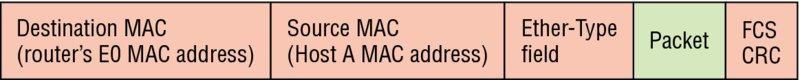
\includegraphics{images/c09f003.jpg}
  \caption{{\protect\hyperlink{c09.xhtmlux5cux23figureanchor9-3}{\textbf{FIGURE
  9.3}} Frame used from Host A to the Lab\_A router when Host B is
  pinged}}
  \end{figure}
\item
  Once the frame is completed, it's handed down to the Physical layer to
  be put on the physical medium (in this example, twisted-pair wire) one
  bit at a time.
\item
  Every device in the collision domain receives these bits and builds
  the frame. They each run a CRC and check the answer in the FCS field.
  If the answers don't match, the frame is discarded.

  \begin{enumerate}
  \tightlist
  \item
    If the CRC matches, then the hardware destination address is checked
    to see if it matches (which, in this example, is the router's
    interface Ethernet 0).
  \item
    If it's a match, then the Ether-Type field is checked to find the
    protocol used at the Network layer.
  \end{enumerate}
\item
  The packet is pulled from the frame, and what is left of the frame is
  discarded. The packet is handed to the protocol listed in the
  Ether-Type field---it's given to IP.
\item
  IP receives the packet and checks the IP destination address. Since
  the packet's destination address doesn't match any of the addresses
  configured on the receiving router itself, the router will look up the
  destination IP network address in its routing table.
\item
  The routing table must have an entry for the network 172.16.20.0 or
  the packet will be discarded immediately and an ICMP message will be
  sent back to the originating device with a destination network
  unreachable message.
\item
  If the router does find an entry for the destination network in its
  table, the packet is switched to the exit interface---in this example,
  interface Ethernet 1. The following output displays the Lab\_A
  router's routing table. The \texttt{C} means ``directly connected.''
  No routing protocols are needed in this network since all networks
  (all two of them) are directly connected.

\begin{verbatim}
Lab_A>sh ip route
C       172.16.10.0 is directly connected,    Ethernet0
L       172.16.10.1/32 is directly connected, Ethernet0
C       172.16.20.0 is directly connected,    Ethernet1
L       172.16.20.1/32 is directly connected, Ethernet1
\end{verbatim}
\item
  \protect\hypertarget{c09.xhtmlux5cux23Page_364}{}{}The router
  packet-switches the packet to the Ethernet 1 buffer.
\item
  The Ethernet 1 buffer needs to know the hardware address of the
  destination host and first checks the ARP cache.

  \begin{enumerate}
  \item
    If the hardware address of Host\_B has already been resolved and is
    in the router's ARP cache, then the packet and the hardware address
    will be handed down to the Data Link layer to be framed. Let's take
    a look at the ARP cache on the Lab\_A router by using the
    \texttt{show\ ip\ arp} command:

\begin{verbatim}
Lab_A#sh ip arp
Protocol  Address     Age(min) Hardware Addr  Type   Interface
Internet  172.16.20.1   -     00d0.58ad.05f4  ARPA   Ethernet1
Internet  172.16.20.2   3     0030.9492.a5dd  ARPA   Ethernet1
Internet  172.16.10.1   -     00d0.58ad.06aa  ARPA   Ethernet0
Internet  172.16.10.2  12     0030.9492.a4ac  ARPA   Ethernet0
\end{verbatim}

    The dash (-) signifies that this is the physical interface on the
    router. This output shows us that the router knows the 172.16.10.2
    (Host\_A) and 172.16.20.2 (Host\_B) hardware addresses. Cisco
    routers will keep an entry in the ARP table for 4 hours.
  \item
    Now if the hardware address hasn't already been resolved, the router
    will send an ARP request out E1 looking for the 172.16.20.2 hardware
    address. Host\_B responds with its hardware address, and the packet
    and destination hardware addresses are then both sent to the Data
    Link layer for framing.
  \end{enumerate}
\item
  The Data Link layer creates a frame with the destination and source
  hardware addresses, Ether-Type field, and FCS field at the end. The
  frame is then handed to the Physical layer to be sent out on the
  physical medium one bit at a time.
\item
  Host\_B receives the frame and immediately runs a CRC. If the result
  matches the information in the FCS field, the hardware destination
  address will then be checked next. If the host finds a match, the
  Ether-Type field is then checked to determine the protocol that the
  packet should be handed to at the Network layer---IP in this example.
\item
  At the Network layer, IP receives the packet and runs a CRC on the IP
  header. If that passes, IP then checks the destination address. Since
  a match has finally been made, the Protocol field is checked to find
  out to whom the payload should be given.
\item
  The payload is handed to ICMP, which understands that this is an echo
  request. ICMP responds to this by immediately discarding the packet
  and generating a new payload as an echo reply.
\item
  A packet is then created including the source and destination
  addresses, Protocol field, and payload. The destination device is now
  Host\_A.
\item
  IP then checks to see whether the destination IP address is a device
  on the local LAN or on a remote network. Since the destination device
  is on a remote network, the packet needs to be sent to the default
  gateway.
\item
  \protect\hypertarget{c09.xhtmlux5cux23Page_365}{}{}The default gateway
  IP address is found in the Registry of the Windows device, and the ARP
  cache is checked to see if the hardware address has already been
  resolved from an IP address.
\item
  Once the hardware address of the default gateway is found, the packet
  and destination hardware addresses are handed down to the Data Link
  layer for framing.
\item
  The Data Link layer frames the packet of information and includes the
  following in the header:

  \begin{enumerate}
  \tightlist
  \item
    The destination and source hardware addresses
  \item
    The Ether-Type field with 0x0800 (IP) in it
  \item
    The FCS field with the CRC result in tow
  \end{enumerate}
\item
  The frame is now handed down to the Physical layer to be sent out over
  the network medium one bit at a time.
\item
  The router's Ethernet 1 interface receives the bits and builds a
  frame. The CRC is run, and the FCS field is checked to make sure the
  answers match.
\item
  Once the CRC is found to be okay, the hardware destination address is
  checked. Since the router's interface is a match, the packet is pulled
  from the frame and the Ether-Type field is checked to determine which
  protocol the packet should be delivered to at the Network layer.
\item
  The protocol is determined to be IP, so it gets the packet. IP runs a
  CRC check on the IP header first and then checks the destination IP
  address.

  \begin{center}\rule{0.5\linewidth}{0.5pt}\end{center}

  %\includegraphics{images/note.png}
  IP does not run a complete CRC as
  the Data Link layer does---it only checks the header for errors.

  \begin{center}\rule{0.5\linewidth}{0.5pt}\end{center}

  Since the IP destination address doesn't match any of the router's
  interfaces, the routing table is checked to see whether it has a route
  to 172.16.10.0. If it doesn't have a route over to the destination
  network, the packet will be discarded immediately. I want to take a
  minute to point out that this is exactly where the source of confusion
  begins for a lot of administrators because when a ping fails, most
  people think the packet never reached the destination host. But as we
  see here, that's not \emph{always} the case. All it takes for this to
  happen is for even just one of the remote routers to lack a route back
  to the originating host's network and--- \emph{poof!}---the packet is
  dropped on the \emph{return trip}, not on its way to the host!

  \begin{center}\rule{0.5\linewidth}{0.5pt}\end{center}

  %\includegraphics{images/tip.png}
  Just a quick note to mention that
  when (and if) the packet is lost on the way back to the originating
  host, you will typically see a request timed-out message because it is
  an unknown error. If the error occurs because of a known issue, such
  as if a route is not in the routing table on the way to the
  destination device, you will see a destination unreachable message.
  This should help you determine if the problem occurred on the way to
  the destination or on the way back.

  \begin{center}\rule{0.5\linewidth}{0.5pt}\end{center}
\item
  \protect\hypertarget{c09.xhtmlux5cux23Page_366}{}{}In this case, the
  router happens to know how to get to network 172.16.10.0---the exit
  interface is Ethernet 0---so the packet is switched to interface
  Ethernet 0.
\item
  The router then checks the ARP cache to determine whether the hardware
  address for 172.16.10.2 has already been resolved.
\item
  Since the hardware address to 172.16.10.2 is already cached from the
  originating trip to Host\_B, the hardware address and packet are then
  handed to the Data Link layer.
\item
  The Data Link layer builds a frame with the destination hardware
  address and source hardware address and then puts IP in the Ether-Type
  field. A CRC is run on the frame and the result is placed in the FCS
  field.
\item
  The frame is then handed to the Physical layer to be sent out onto the
  local network one bit at a time.
\item
  The destination host receives the frame, runs a CRC, checks the
  destination hardware address, then looks into the Ether-Type field to
  find out to whom to hand the packet.
\item
  IP is the designated receiver, and after the packet is handed to IP at
  the Network layer, it checks the Protocol field for further direction.
  IP finds instructions to give the payload to ICMP, and ICMP determines
  the packet to be an ICMP echo reply.
\item
  ICMP acknowledges that it has received the reply by sending an
  exclamation point (!) to the user interface. ICMP then attempts to
  send four more echo requests to the destination host.
\end{enumerate}

You've just experienced Todd's 36 easy steps to understanding IP
routing. The key point here is that if you had a much larger network,
the process would be the \emph{same}. It's just that the larger the
internetwork, the more hops the packet goes through before it finds the
destination host.

It's super-important to remember that when Host\_A sends a packet to
Host\_B, the destination hardware address used is the default gateway's
Ethernet interface. Why? Because frames can't be placed on remote
networks---only local networks. So packets destined for remote networks
must go through the default gateway.

Let's take a look at Host\_A's ARP cache now:

\begin{verbatim}
C:\ >arp -a
Interface: 172.16.10.2 --- 0x3
  Internet Address      Physical Address      Type
  172.16.10.1           00-15-05-06-31-b0     dynamic
  172.16.20.1           00-15-05-06-31-b0     dynamic
\end{verbatim}

Did you notice that the hardware (MAC) address that Host\_A uses to get
to Host\_B is the Lab\_A E0 interface? Hardware addresses are
\emph{always} local, and they never pass through a router's interface.
Understanding this process is as important as air to you, so carve this
into your memory!

\subsubsection[The Cisco Router Internal
Process]{\texorpdfstring{\protect\hypertarget{c09.xhtmlux5cux23c09-sec-3}{}{}The
Cisco Router Internal Process}{The Cisco Router Internal Process}}

One more thing before we get to testing your understanding of my 36
steps of IP routing. I think it's important to explain how a router
forwards packets internally. For IP to look up a
\protect\hypertarget{c09.xhtmlux5cux23Page_367}{}{}destination address
in a routing table on a router, processing in the router must take
place, and if there are tens of thousands of routes in that table, the
amount of CPU time would be enormous. It results in a potentially
overwhelming amount of overhead---think about a router at your ISP that
has to calculate millions of packets per second and even subnet to find
the correct exit interface! Even with the little network I'm using in
this book, lots of processing would need to be done if there were actual
hosts connected and sending data.

Cisco uses three types of packet-forwarding techniques.

\textbf{Process switching} This is actually how many people see routers
to this day, because it's true that routers actually did perform this
type of bare-bones packet switching back in 1990 when Cisco released
their very first router. But those days when traffic demands were
unimaginably light are long gone---not in today's networks! This process
is now extremely complex and involves looking up every destination in
the routing table and finding the exit interface for every packet. This
is pretty much how I just explained the process in my 36 steps. But even
though what I wrote was absolutely true in concept, the internal process
requires much more than packet-switching technology today because of the
millions of packets per second that must now be processed. So Cisco came
up with some other technologies to help with the ``big process
problem.''

\textbf{Fast switching} This solution was created to make the slow
performance of process switching faster and more efficient. Fast
switching uses a cache to store the most recently used destinations so
that lookups are not required for every packet. By caching the exit
interface of the destination device, as well as the layer 2 header,
performance was dramatically improved, but as our networks evolved with
the need for even more speed, Cisco created yet another technology!

\textbf{Cisco Express Forwarding (CEF)} This is Cisco's newer creation,
and it's the default packet-forwarding method used on all the latest
Cisco routers. CEF makes many different cache tables to help improve
performance and is change triggered, not packet triggered. Translated,
this means that when the network topology changes, the cache changes
along with it.

\begin{center}\rule{0.5\linewidth}{0.5pt}\end{center}

%\includegraphics{images/tip.png}
To see which packet switching method
your router interface is using, use the command
\texttt{show\ ip\ interface}.

\begin{center}\rule{0.5\linewidth}{0.5pt}\end{center}

\subsubsection[Testing Your IP Routing
Understanding]{\texorpdfstring{\protect\hypertarget{c09.xhtmlux5cux23c09-sec-4}{}{}Testing
Your IP Routing Understanding}{Testing Your IP Routing Understanding}}

Since understanding IP routing is super-important, it's time for that
little test I talked about earlier on how well you've got the IP routing
process down so far. I'm going to do that by having you look at a couple
of figures and answer some very basic IP routing questions based upon
them.

\protect\hyperlink{c09.xhtmlux5cux23figure9-4}{Figure 9.4} shows a LAN
connected to RouterA that's connected via a WAN link to RouterB. RouterB
has a LAN connected with an HTTP server attached.

\protect\hypertarget{c09.xhtmlux5cux23Page_368}{}{}

\begin{figure}
\centering
%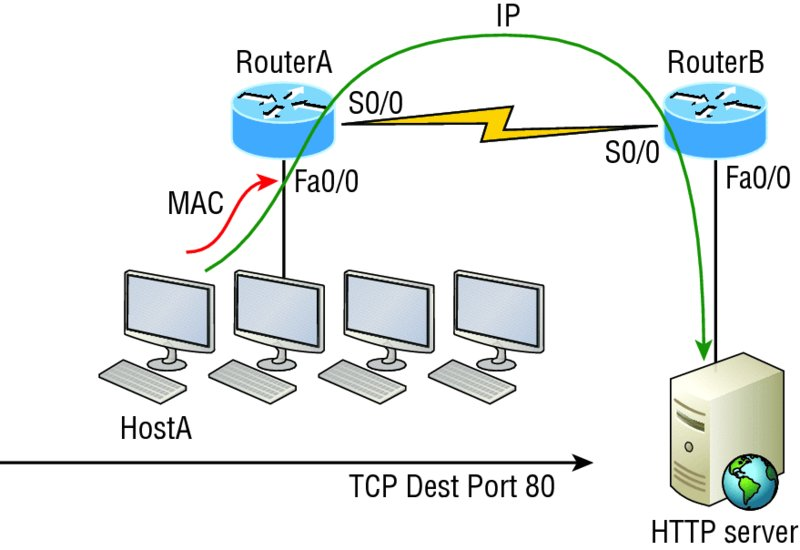
\includegraphics{images/c09f004.jpg}
\caption{{\protect\hyperlink{c09.xhtmlux5cux23figureanchor9-4}{\textbf{FIGURE
9.4}} IP routing example 1}}
\end{figure}

The critical information you want to obtain by looking at this figure is
exactly how IP routing will occur in this example. Let's determine the
characteristics of a frame as it leaves HostA. Okay---we'll cheat a bit.
I'll give you the answer, but then you should go back over the figure
and see if you can answer example 2 without looking at my three-step
answer!

\begin{enumerate}
\tightlist
\item
  The destination address of a frame from HostA would be the MAC address
  of Router A's Fa0/0 interface.
\item
  The destination address of a packet would be the IP address of the
  HTTP server's network interface card (NIC).
\item
  The destination port number in the segment header would be 80.
\end{enumerate}

That was a pretty simple, straightforward scenario. One thing to
remember is that when multiple hosts are communicating to a server using
HTTP, they must all use a different source port number. The source and
destination IP addresses and port numbers are how the server keeps the
data separated at the Transport layer.

Let's complicate matters by adding another device into the network and
then see if you can find the answers.
\protect\hyperlink{c09.xhtmlux5cux23figure9-5}{Figure 9.5} shows a
network with only one router but two switches.

\begin{figure}
\centering
%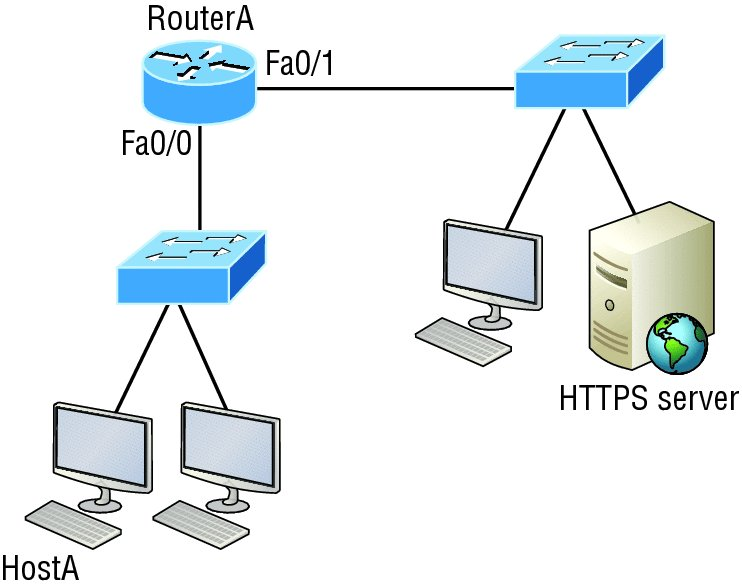
\includegraphics{images/c09f005.jpg}
\caption{{\protect\hyperlink{c09.xhtmlux5cux23figureanchor9-5}{\textbf{FIGURE
9.5}} IP routing example 2}}
\end{figure}

\protect\hypertarget{c09.xhtmlux5cux23Page_369}{}{}The key thing to
understand about the IP routing process in this scenario is what happens
when HostA sends data to the HTTPS server? Here's your answer:

\begin{enumerate}
\tightlist
\item
  The destination address of a frame from HostA would be the MAC address
  of RouterA's Fa0/0 interface.
\item
  The destination address of a packet is the IP address of the HTTPS
  server's network interface card (NIC).
\item
  The destination port number in the segment header will have a value of
  443.
\end{enumerate}

Did you notice that the switches weren't used as either a default
gateway or any other destination? That's because switches have nothing
to do with routing. I wonder how many of you chose the switch as the
default gateway (destination) MAC address for HostA? If you did, don't
feel bad---just take another look to see where you went wrong and why.
It's very important to remember that the destination MAC address will
always be the router's interface---if your packets are destined for
outside the LAN, as they were in these last two examples!

Before moving on into some of the more advanced aspects of IP routing,
let's look at another issue. Take a look at the output of this router's
routing table:

\begin{verbatim}
Corp#sh ip route
[output cut]
R    192.168.215.0 [120/2] via 192.168.20.2, 00:00:23, Serial0/0
R    192.168.115.0 [120/1] via 192.168.20.2, 00:00:23, Serial0/0
R    192.168.30.0 [120/1] via 192.168.20.2, 00:00:23, Serial0/0
C    192.168.20.0 is directly connected, Serial0/0
L    192.168.20.1/32 is directly connected, Serial0/0
C    192.168.214.0 is directly connected, FastEthernet0/0
L    192.168.214.1/32 is directly connected, FastEthernet0/0
\end{verbatim}

What do we see here? If I were to tell you that the corporate router
received an IP packet with a source IP address of 192.168.214.20 and a
destination address of 192.168.22.3, what do you think the Corp router
will do with this packet?

If you said, ``The packet came in on the FastEthernet 0/0 interface, but
because the routing table doesn't show a route to network 192.168.22.0
(or a default route), the router will discard the packet and send an
ICMP destination unreachable message back out to interface FastEthernet
0/0,'' you're a genius! The reason that's the correct answer is because
that's the source LAN where the packet originated from.

Now, let's check out the next figure and talk about the frames and
packets in detail. We're not really going over anything new here; I'm
just making sure you totally, completely, thoroughly, fully understand
basic IP routing! It is the crux of this book, and the topic the exam
objectives are geared toward. It's all about IP routing, which means you
need to be all over this stuff! We'll use
\protect\hyperlink{c09.xhtmlux5cux23figure9-6}{Figure 9.6} for the next
few scenarios.

\protect\hypertarget{c09.xhtmlux5cux23Page_370}{}{}

\begin{figure}
\centering
%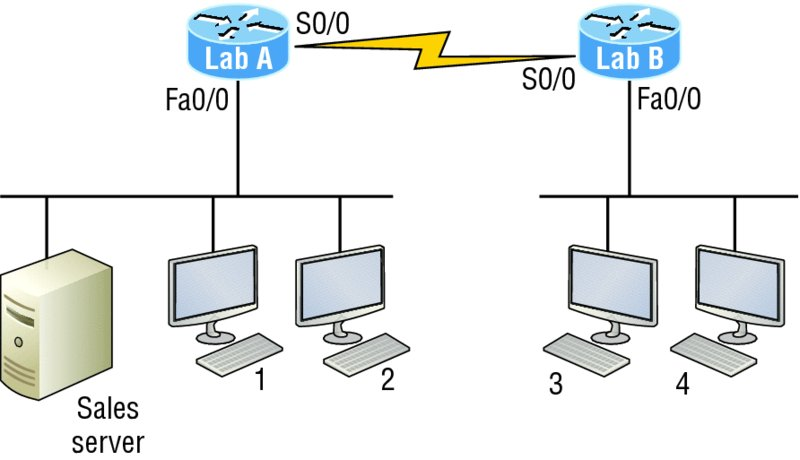
\includegraphics{images/c09f006.jpg}
\caption{{\protect\hyperlink{c09.xhtmlux5cux23figureanchor9-6}{\textbf{FIGURE
9.6}} Basic IP routing using MAC and IP addresses}}
\end{figure}

Referring to \protect\hyperlink{c09.xhtmlux5cux23figure9-6}{Figure 9.6},
here's a list of all the answers to questions you need inscribed in your
brain:

\begin{enumerate}
\tightlist
\item
  In order to begin communicating with the Sales server, Host 4 sends
  out an ARP request. How will the devices exhibited in the topology
  respond to this request?
\item
  Host 4 has received an ARP reply. Host 4 will now build a packet, then
  place this packet in the frame. What information will be placed in the
  header of the packet that leaves Host 4 if Host 4 is going to
  communicate to the Sales server?
\item
  The Lab\_A router has received the packet and will send it out Fa0/0
  onto the LAN toward the server. What will the frame have in the header
  as the source and destination addresses?
\item
  Host 4 is displaying two web documents from the Sales server in two
  browser windows at the same time. How did the data find its way to the
  correct browser windows?
\end{enumerate}

The following should probably be written in a teensy font and put upside
down in another part of the book so it would be really hard for you to
cheat and peek, but since I'm not that mean and you really need to have
this down, here are your answers in the same order that the scenarios
were just presented:

\begin{enumerate}
\tightlist
\item
  In order to begin communicating with the server, Host 4 sends out an
  ARP request. How will the devices exhibited in the topology respond to
  this request? Since MAC addresses must stay on the local network, the
  Lab\_B router will respond with the MAC address of the Fa0/0 interface
  and Host 4 will send all frames to the MAC address of the Lab\_B Fa0/0
  interface when sending packets to the Sales server.
\item
  Host 4 has received an ARP reply. Host 4 will now build a packet, then
  place this packet in the frame. What information will be placed in the
  header of the packet that leaves Host 4 if Host 4 is going to
  communicate to the Sales server? Since we're now talking about
  packets, not frames, the source address will be the IP address of Host
  4 and the destination address will be the IP address of the Sales
  server.
\item
  Finally, the Lab\_A router has received the packet and will send it
  out Fa0/0 onto the LAN toward the server. What will the frame have in
  the header as the source and ­destination addresses? The source MAC
  address will be the Lab\_A router's Fa0/0 interface, and the
  \protect\hypertarget{c09.xhtmlux5cux23Page_371}{}{}destination MAC
  address will be the Sales server's MAC address because all MAC
  addresses must be local on the LAN.
\item
  Host 4 is displaying two web documents from the Sales server in two
  different browser windows at the same time. How did the data find its
  way to the correct browser windows? TCP port numbers are used to
  direct the data to the correct application window.
\end{enumerate}

Great! But we're not quite done yet. I've got a few more questions for
you before you actually get to configure routing in a real network.
Ready? \protect\hyperlink{c09.xhtmlux5cux23figure9-7}{Figure 9.7} shows
a basic network, and Host 4 needs to get email. Which address will be
placed in the destination address field of the frame when it leaves Host
4?

\begin{figure}
\centering
%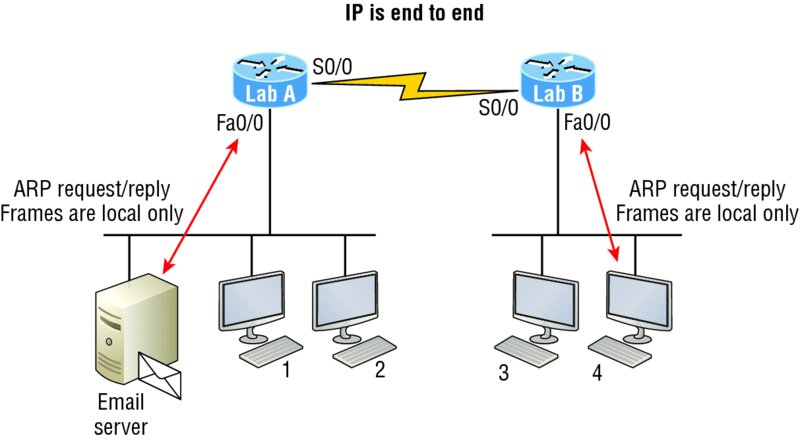
\includegraphics{images/c09f007.jpg}
\caption{{\protect\hyperlink{c09.xhtmlux5cux23figureanchor9-7}{\textbf{FIGURE
9.7}} Testing basic routing knowledge}}
\end{figure}

The answer is that Host 4 will use the destination MAC address of the
Fa0/0 interface on the Lab\_B router---you knew that, right? Look at
\protect\hyperlink{c09.xhtmlux5cux23figure9-7}{Figure 9.7} again: What
if Host 4 needs to communicate with Host 1---not the server, but with
Host 1. Which OSI layer 3 source address will be found in the packet
header when it reaches Host 1?

Hopefully you've got this: At layer 3, the source IP address will be
Host 4 and the destination address in the packet will be the IP address
of Host 1. Of course, the destination MAC address from Host 4 will
always be the Fa0/0 address of the Lab\_B router, right? And since we
have more than one router, we'll need a routing protocol that
communicates between both of them so that traffic can be forwarded in
the right direction to reach the network that Host 1 is connected to.

Okay---one more scenario and you're on your way to being an IP routing
machine! Again, using
\protect\hyperlink{c09.xhtmlux5cux23figure9-7}{Figure 9.7}, Host 4 is
transferring a file to the email server connected to the Lab\_A router.
What would be the layer 2 destination address leaving Host 4? Yes, I've
asked this question more than once. But not this one: What will be the
source MAC address when the frame is received at the email server?

\protect\hypertarget{c09.xhtmlux5cux23Page_372}{}{}Hopefully, you
answered that the layer 2 destination address leaving Host 4 is the MAC
address of the Fa0/0 interface on the Lab\_B router and that the source
layer 2 address that the email server will receive is the Fa0/0
interface of the Lab\_A router.

If you did, you're ready to discover how IP routing is handled in a
larger network environment!




\section{Configuring IP Routing}

It's time to get serious and configure a real network.
\protect\hyperlink{c09.xhtmlux5cux23figure9-8}{Figure 9.8} shows three
routers: Corp, SF, and LA. Remember that, by default, these routers only
know about networks that are directly connected to them. I'll continue
to use this figure and network throughout the rest of the chapters in
this book. As I progress through this book, I'll add more routers and
switches as needed.

\begin{figure}
\centering
%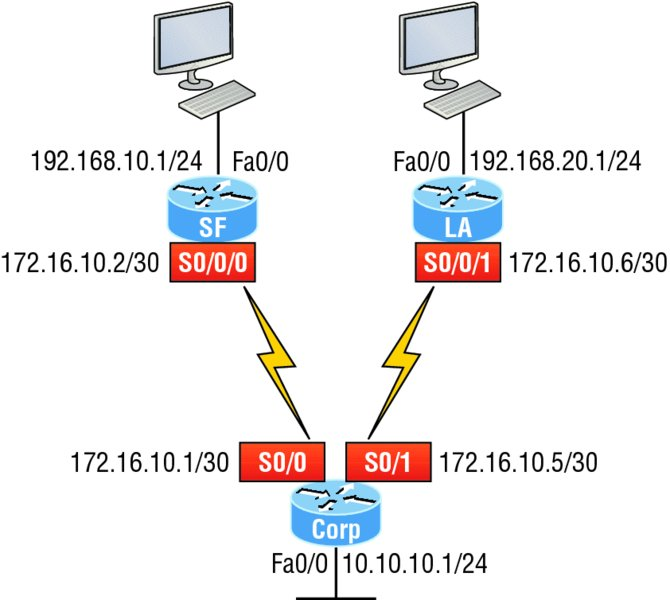
\includegraphics{images/c09f008.jpg}
\caption{{\protect\hyperlink{c09.xhtmlux5cux23figureanchor9-8}{\textbf{FIGURE
9.8}} Configuring IP routing}}
\end{figure}

As you might guess, I've got quite a nice collection of routers for us
to play with. But you don't need a closet full of devices to perform
most, if not all, of the commands we'll use in this book. You can get by
nicely with pretty much any router or even with a good router simulator.

Getting back to business, the Corp router has two serial interfaces,
which will provide a WAN connection to the SF and LA router and two Fast
Ethernet interfaces as well. The two remote routers have two serial
interfaces and two Fast Ethernet interfaces.

The first step for this project is to correctly configure each router
with an IP address on each interface. The following list shows the IP
address scheme I'm going to use to configure the network. After we go
over how the network is configured, I'll cover how to configure
\protect\hypertarget{c09.xhtmlux5cux23Page_373}{}{}IP routing. Pay
attention to the subnet masks---they're important! The LANs all use a
/24 mask, but the WANs are using a /30.

Corp

\begin{enumerate}
\tightlist
\item
  Serial 0/0: 172.16.10.1/30
\item
  Serial 0/1: 172.16.10.5/30
\item
  Fa0/0: 10.10.10.1/24
\end{enumerate}

SF

\begin{enumerate}
\tightlist
\item
  S0/0/0: 172.16.10.2/30
\item
  Fa0/0: 192.168.10.1/24
\end{enumerate}

LA

\begin{enumerate}
\tightlist
\item
  S0/0/0: 172.16.10.6/30
\item
  Fa0/0: 192.168.20.1/24
\end{enumerate}

The router configuration is really a pretty straightforward process
since you just need to add IP addresses to your interfaces and then
perform a \texttt{no\ shutdown} on those same interfaces. It gets a tad
more complex later on, but for right now, let's configure the IP
addresses in the network.

\subsubsection[Corp
Configuration]{\texorpdfstring{\protect\hypertarget{c09.xhtmlux5cux23c09-sec-6}{}{}Corp
Configuration}{Corp Configuration}}

We need to configure three interfaces to configure the Corp router. And
configuring the hostnames of each router will make identification much
easier. While we're at it, let's set the interface descriptions, banner,
and router passwords too because it's a really good idea to make a habit
of configuring these commands on every router!

To get started, I performed an \texttt{erase\ startup-config} on the
router and reloaded, so we'll start in setup mode. I chose \texttt{no}
when prompted to enter setup mode, which will get us straight to the
username prompt of the console. I'm going to configure all my routers
this same way.

Here's how what I just did looks:

\begin{verbatim}
         --- System Configuration Dialog ---
Would you like to enter the initial configuration dialog? [yes/no]: n
 
Press RETURN to get started!
Router>en
Router#config t
Router(config)#hostname Corp
Corp(config)#enable secret GlobalNet
Corp(config)#no ip domain-lookup
Corp(config)#int f0/0
Corp(config-if)#desc Connection to LAN BackBone
Corp(config-if)#ip address 10.10.10.1 255.255.255.0
Corp(config-if)#no shut
Corp(config-if)#int s0/0
Corp(config-if)#desc WAN connection to SF
Corp(config-if)#ip address 172.16.10.1 255.255.255.252
Corp(config-if)#no shut
Corp(config-if)#int s0/1
Corp(config-if)#desc WAN connection to LA
Corp(config-if)#ip address 172.16.10.5 255.255.255.252
Corp(config-if)#no shut
Corp(config-if)#line con 0
Corp(config-line)#password console
Corp(config-line)#logging
Corp(config-line)#logging sync
Corp(config-line)#exit
Corp(config)#line vty 0 ?
  <1-181>  Last Line number
  <cr>
Corp(config)#line vty 0 181
Corp(config-line)#password telnet
Corp(config-line)#login
Corp(config-line)#exit
Corp(config)#banner motd # This is my Corp Router #
Corp(config)#^Z
Corp#copy run start
Destination filename [startup-config]?
Building configuration...
[OK]
Corp# [OK]
\end{verbatim}

Let's talk about the configuration of the Corp router. First, I set the
hostname and enable secret, but what is that
\texttt{no\ ip\ domain-lookup} command? That command stops the router
from trying to resolve hostnames, which is an annoying feature unless
you've configured a host table or DNS. Next, I configured the three
interfaces with descriptions and IP addresses and enabled them with the
\texttt{no\ shutdown} command. The console and VTY passwords came next,
but what is that \texttt{logging\ sync} command under the console line?
The logging synchronous command stops console messages from writing over
what you are typing in, meaning it's a sanity-saving command that you'll
come to love! Last, I set my banner and then saved my configs.

\begin{center}\rule{0.5\linewidth}{0.5pt}\end{center}

%\includegraphics{images/note.png}
If you're having a hard time
understanding this configuration process, refer back to Chapter 6,
``Cisco's Internetworking Operating System (IOS).''

\begin{center}\rule{0.5\linewidth}{0.5pt}\end{center}

\protect\hypertarget{c09.xhtmlux5cux23Page_375}{}{}To view the IP
routing tables created on a Cisco router, use the command
\texttt{show\ ip\ route}. Here's the command's output:

\begin{verbatim}
Corp#sh ip route
Codes: L - local, C - connected, S - static, R - RIP, M - mobile, B - BGP
   D - EIGRP, EX - EIGRP external, O - OSPF, IA - OSPF inter area
   N1 - OSPF NSSA external type 1, N2 - OSPF NSSA external type 2
   E1 - OSPF external type 1, E2 - OSPF external type 2
   i - IS-IS, su - IS-IS summary, L1 - IS-IS level-1, L2 - IS-IS level-2
   ia - IS-IS inter area, * - candidate default, U - per-user static route
   o - ODR, P - periodic downloaded static route, H - NHRP, l - LISP
   + - replicated route, % - next hop override
Gateway of last resort is not set
 
     10.0.0.0/24 is subnetted, 1 subnets
C       10.10.10.0 is directly connected, FastEthernet0/0
L       10.10.10.1/32 is directly connected, FastEthernet0/0
Corp#
\end{verbatim}

It's important to remember that only configured, directly connected
networks are going to show up in the routing table. So why is it that
only the FastEthernet 0/0 interface shows up in the table? No
worries---that's just because you won't see the serial interfaces come
up until the other side of the links are operational. As soon as we
configure our SF and LA routers, those interfaces should pop right up!

But did you notice the \texttt{C} on the left side of the output of the
routing table? When you see that there, it means that the network is
directly connected. The codes for each type of connection are listed at
the top of the \texttt{show\ ip\ route} command, along with their
descriptions.

\begin{center}\rule{0.5\linewidth}{0.5pt}\end{center}

%\includegraphics{images/note.png}
For brevity, the codes at the top of
the output will be cut in the rest of this chapter.

\begin{center}\rule{0.5\linewidth}{0.5pt}\end{center}

\subsubsection[SF
Configuration]{\texorpdfstring{\protect\hypertarget{c09.xhtmlux5cux23c09-sec-7}{}{}SF
Configuration}{SF Configuration}}

Now we're ready to configure the next router---SF. To make that happen
correctly, keep in mind that we have two interfaces to deal with: Serial
0/0/0 and FastEthernet 0/0. So let's make sure we don't forget to add
the hostname, passwords, interface descriptions, and banners to the
router configuration. As I did with the Corp router, I erased the
configuration and reloaded since this router had already been configured
before.

Here's the configuration I used:

\begin{verbatim}
R1#erase start
% Incomplete command.
R1#erase startup-config
Erasing the nvram filesystem will remove all configuration files!
   Continue? [confirm][enter]
[OK]
Erase of nvram: complete
R1#reload
Proceed with reload? [confirm][enter]
[output cut]
%Error opening tftp://255.255.255.255/network-confg (Timed out)
%Error opening tftp://255.255.255.255/cisconet.cfg (Timed out)
 
         --- System Configuration Dialog ---
 
Would you like to enter the initial configuration dialog? [yes/no]: n
\end{verbatim}

Before we move on, let's talk about this output for a second. First,
notice that beginning with IOS 12.4, ISR routers will no longer take the
command \texttt{erase\ start}. The router has only one command after
\texttt{erase} that starts with \emph{s}, as shown here:

\begin{verbatim}
Router#erase s?
startup-config
\end{verbatim}

I know, you'd think that the IOS would continue to accept the command,
but nope---sorry! The second thing I want to point out is that the
output tells us the router is looking for a TFTP host to see if it can
download a configuration. When that fails, it goes straight into setup
mode. This gives you a great picture of the Cisco router default boot
sequence we talked about in Chapter 7, ``Managing a Cisco
Internetwork.''

Let's get back to configuring our router:

\begin{verbatim}
Press RETURN to get started!
Router#config t
Router(config)#hostname SF
SF(config)#enable secret GlobalNet
SF(config)#no ip domain-lookup
SF(config)#int s0/0/0
SF(config-if)#desc WAN Connection to Corp
SF(config-if)#ip address 172.16.10.2 255.255.255.252
SF(config-if)#no shut
SF(config-if)#clock rate 1000000
SF(config-if)#int f0/0
SF(config-if)#desc SF LAN
SF(config-if)#ip address 192.168.10.1 255.255.255.0
SF(config-if)#no shut
SF(config-if)#line con 0
SF(config-line)#password console
SF(config-line)#login
SF(config-line)#logging sync
SF(config-line)#exit
SF(config)#line vty 0 ?
  <1-1180>  Last Line number
  <cr>
SF(config)#line vty 0 1180
SF(config-line)#password telnet
SF(config-line)#login
SF(config-line)#banner motd #This is the SF Branch router#
SF(config)#exit
SF#copy run start
Destination filename [startup-config]?
Building configuration...
 [OK]
\end{verbatim}

Let's take a look at our configuration of the interfaces with the
following two commands:

\begin{verbatim}
SF#sh run | begin int
interface FastEthernet0/0
 description SF LAN
 ip address 192.168.10.1 255.255.255.0
 duplex auto
 speed auto
!
interface FastEthernet0/1
 no ip address
 shutdown
 duplex auto
 speed auto
!
interface Serial0/0/0
 description WAN Connection to Corp
 ip address 172.16.10.2 255.255.255.252
 clock rate 1000000
!
SF#sh ip int brief
Interface             IP-Address      OK? Method Status                Protocol
FastEthernet0/0       192.168.10.1    YES manual up                    up
FastEthernet0/1       unassigned      YES unset  administratively down down
Serial0/0/0           172.16.10.2     YES manual up                    up
Serial0/0/1           unassigned      YES unset  administratively down down
SF#
\end{verbatim}

Now that both ends of the serial link are configured, the link comes up.
Remember, the up/up status for the interfaces are Physical/Data Link
layer status indicators that don't reflect the layer 3 status! I ask
students in my classes, ``If the link shows up/up, can you ping the
directly connected network?'' And they say, ``Yes!'' The correct answer
is, ``I don't know,'' because we can't see the layer 3 status with this
command. We only see layers 1 and 2 and verify that the IP addresses
don't have a typo. This is really important to understand!

The \texttt{show\ ip\ route} command for the SF router reveals the
following:

\begin{verbatim}
SF#sh ip route
C    192.168.10.0/24 is directly connected, FastEthernet0/0
L    192.168.10.1/32 is directly connected, FastEthernet0/0
     172.16.0.0/30 is subnetted, 1 subnets
C       172.16.10.0 is directly connected, Serial0/0/0
L       172.16.10.2/32 is directly connected, Serial0/0/0
\end{verbatim}

Notice that router SF knows how to get to networks 172.16.10.0/30 and
192.168.10.0/24; we can now ping to the Corp router from SF:

\begin{verbatim}
SF#ping 172.16.10.1
 
Type escape sequence to abort.
Sending 5, 100-byte ICMP Echos to 172.16.10.1, timeout is 2 seconds:
!!!!!
Success rate is 100 percent (5/5), round-trip min/avg/max = 1/3/4 ms
\end{verbatim}

Now let's head back to the Corp router and check out the routing table:

\begin{verbatim}
Corp>sh ip route
     172.16.0.0/30 is subnetted, 1 subnets
C       172.16.10.0 is directly connected, Serial0/0
L       172.16.10.1/32 is directly connected, Serial0/0
     10.0.0.0/24 is subnetted, 1 subnets
C       10.10.10.0 is directly connected, FastEthernet0/0
L       10.10.10.1/32 is directly connected, FastEthernet0/0
\end{verbatim}

On the SF router's serial interface 0/0/0 is a DCE connection, which
means a clock rate needs to be set on the interface. Remember that you
don't need to use the \texttt{clock\ rate} command in production. While
true, it's still imperative that you know how/when you can use it and
that you understand it really well when studying for your CCNA exam!

\protect\hypertarget{c09.xhtmlux5cux23Page_379}{}{}We can see our
clocking with the \texttt{show\ controllers} command:

\begin{verbatim}
SF#sh controllers s0/0/0
Interface Serial0/0/0
Hardware is GT96K
DCE V.35, clock rate 1000000

Corp>sh controllers s0/0
Interface Serial0/0
Hardware is PowerQUICC MPC860
DTE V.35 TX and RX clocks detected.
\end{verbatim}

Since the SF router has a DCE cable connection, I needed to add clock
rate to this interface because DTE receives clock. Keep in mind that the
new ISR routers will autodetect this and set the clock rate to 2000000.
And you still need to make sure you're able to find an interface that is
DCE and set clocking to meet the objectives.

Since the serial links are showing up, we can now see both networks in
the Corp routing table. And once we configure LA, we'll see one more
network in the routing table of the Corp router. The Corp router can't
see the 192.168.10.0 network because we don't have any routing
configured yet---routers see only directly connected networks by
default.

\subsubsection[LA
Configuration]{\texorpdfstring{\protect\hypertarget{c09.xhtmlux5cux23c09-sec-8}{}{}LA
Configuration}{LA Configuration}}

To configure LA, we're going to do pretty much the same thing we did
with the other two routers. There are two interfaces to deal with,
Serial 0/0/1 and FastEthernet 0/0, and again, we'll be sure to add the
hostname, passwords, interface descriptions, and a banner to the router
configuration:

\begin{verbatim}
Router(config)#hostname LA
LA(config)#enable secret GlobalNet
LA(config)#no ip domain-lookup
LA(config)#int s0/0/1
LA(config-if)#ip address 172.16.10.6 255.255.255.252
LA(config-if)#no shut
LA(config-if)#clock rate 1000000
LA(config-if)#description WAN To Corporate
LA(config-if)#int f0/0
LA(config-if)#ip address 192.168.20.1 255.255.255.0
LA(config-if)#no shut
LA(config-if)#description LA LAN
LA(config-if)#line con 0
LA(config-line)#password console
LA(config-line)#login
LA(config-line)#logging sync
LA(config-line)#exit
LA(config)#line vty 0 ?
  <1-1180>  Last Line number
  <cr>
LA(config)#line vty 0 1180
LA(config-line)#password telnet
LA(config-line)#login
LA(config-line)#exit
LA(config)#banner motd #This is my LA Router#
LA(config)#exit
LA#copy run start
Destination filename [startup-config]?
Building configuration...
[OK]
\end{verbatim}

Nice---everything was pretty straightforward. The following output,
which I gained via the \texttt{show\ ip\ route} command, displays the
directly connected networks of 192.168.20.0 and 172.16.10.0:

\begin{verbatim}
LA#sh ip route
     172.16.0.0/30 is subnetted, 1 subnets
C       172.16.10.4 is directly connected, Serial0/0/1
L       172.16.10.6/32 is directly connected, Serial0/0/1
C    192.168.20.0/24 is directly connected, FastEthernet0/0
L    192.168.20.1/32 is directly connected, FastEthernet0/0
\end{verbatim}

So now that we've configured all three routers with IP addresses and
administrative functions, we can move on to deal with routing. But I
want to do one more thing on the SF and LA routers---since this is a
very small network, let's build a DHCP server on the Corp router for
each LAN.

\paragraph{Configuring DHCP on Our Corp Router}

While it's true that I could approach this task by going to each remote
router and creating a pool, why bother with all that when I can easily
create two pools on the Corp router and have the remote routers forward
requests to the Corp router? Of course, you remember how to do this from
Chapter 7!

Let's give it a shot:

\begin{verbatim}
Corp#config t
Corp(config)#ip dhcp excluded-address 192.168.10.1
Corp(config)#ip dhcp excluded-address 192.168.20.1
Corp(config)#ip dhcp pool SF_LAN
Corp(dhcp-config)#network 192.168.10.0 255.255.255.0
Corp(dhcp-config)#default-router 192.168.10.1
Corp(dhcp-config)#dns-server 4.4.4.4
Corp(dhcp-config)#exit
Corp(config)#ip dhcp pool LA_LAN
Corp(dhcp-config)#network 192.168.20.0 255.255.255.0
Corp(dhcp-config)#default-router 192.168.20.1
Corp(dhcp-config)#dns-server 4.4.4.4
Corp(dhcp-config)#exit
Corp(config)#exit
Corp#copy run start
Destination filename [startup-config]?
Building configuration...
\end{verbatim}

Creating DHCP pools on a router is actually a simple process, and you
would go about the configuration the same way on any router you wish to
add a DHCP pool to. To designate a router as a DHCP server, you just
create the pool name, add the network/subnet and the default gateway,
and then exclude any addresses that you don't want handed out. You
definitely want to make sure you've excluded the default gateway
address, and you'd usually add a DNS server as well. I always add any
exclusions first, and remember that you can conveniently exclude a range
of addresses on a single line. Soon, I'll demonstrate those verification
commands I promised I'd show you back in Chapter 7, but first, we need
to figure out why the Corp router still can't get to the remote networks
by default!

Now I'm pretty sure I configured DHCP correctly, but I just have this
nagging feeling I forgot something important. What could that be? Well,
the hosts are remote across a router, so what would I need to do that
would allow them to get an address from a DHCP server? If you concluded
that I've got to configure the SF and LA F0/0 interfaces to forward the
DHCP client requests to the server, you got it!

Here's how we'd go about doing that:

\begin{verbatim}
LA#config t
LA(config)#int f0/0
LA(config-if)#ip helper-address 172.16.10.5

SF#config t
SF(config)#int f0/0
SF(config-if)#ip helper-address 172.16.10.1
\end{verbatim}

I'm pretty sure I did this correctly, but we won't know until I have
some type of routing configured and working. So let's get to that next!



\section{Configuring IP Routing in Our Network}

So is our network really good to go? After all, I've configured it with
IP addressing, administrative functions, and even clocking that will
automatically occur with the ISR routers. But how will our routers send
packets to remote networks when they get their destination
\protect\hypertarget{c09.xhtmlux5cux23Page_382}{}{}information by
looking into their tables that only include directions about directly
connected networks? And you know routers promptly discard packets they
receive with addresses for networks that aren't listed in their routing
table!

So we're not exactly ready to rock after all. But we will be soon
because there are several ways to configure the routing tables to
include all the networks in our little internetwork so that packets will
be properly forwarded. As usual, one size fits all rarely fits at all,
and what's best for one network isn't necessarily what's best for
another. That's why understanding the different types of routing will be
really helpful when choosing the best solution for your specific
environment and business requirements.

These are the three routing methods I'm going to cover with you:

\begin{enumerate}
\tightlist
\item
  Static routing
\item
  Default routing
\item
  Dynamic routing
\end{enumerate}

We're going to start with the first way and implement static routing on
our network, because if you can implement static routing \emph{and} make
it work, you've demonstrated that you definitely have a solid
understanding of the internetwork. So let's get started.

\subsubsection[Static
Routing]{\texorpdfstring{\protect\hypertarget{c09.xhtmlux5cux23c09-sec-10}{}{}Static
Routing}{Static Routing}}

Static routing is the process that ensues when you manually add routes
in each router's routing table. Predictably, there are pros and cons to
static routing, but that's true for all routing approaches.

Here are the pros:

\begin{enumerate}
\tightlist
\item
  There is no overhead on the router CPU, which means you could probably
  make do with a cheaper router than you would need for dynamic routing.
\item
  There is no bandwidth usage between routers, saving you money on WAN
  links as well as minimizing overhead on the router since you're not
  using a routing protocol.
\item
  It adds security because you, the administrator, can be very exclusive
  and choose to allow routing access to certain networks only.
\end{enumerate}

And here are the cons:

\begin{enumerate}
\tightlist
\item
  Whoever the administrator is must have a vault-tight knowledge of the
  internetwork and how each router is connected in order to configure
  routes correctly. If you don't have a good, accurate map of your
  internetwork, things will get very messy quickly!
\item
  If you add a network to the internetwork, you have to tediously add a
  route to it on all routers by hand, which only gets increasingly
  insane as the network grows.
\item
  Due to the last point, it's just not feasible to use it in most large
  networks because maintaining it would be a full-time job in itself.
\end{enumerate}

But that list of cons doesn't mean you get to skip learning all about it
mainly because of that first disadvantage I listed---the fact that you
must have such a solid understanding of a network to configure it
properly and that your administrative knowledge has to practically
\protect\hypertarget{c09.xhtmlux5cux23Page_383}{}{}verge on the
supernatural! So let's dive in and develop those skills. Starting at the
beginning, here's the command syntax you use to add a static route to a
routing table from global config:

\begin{verbatim}
ip route [destination_network] [mask] [next-hop_address or
  exitinterface] [administrative_distance] [permanent]
\end{verbatim}

This list describes each command in the string:

\texttt{ip\ route} The command used to create the static route.

\texttt{destination\_network} The network you're placing in the routing
table.

\texttt{mask} The subnet mask being used on the network.

\texttt{next-hop\_address} This is the IP address of the next-hop router
that will receive packets and forward them to the remote network, which
must signify a router interface that's on a directly connected network.
You must be able to successfully ping the router interface before you
can add the route. Important note to self is that if you type in the
wrong next-hop address or the interface to the correct router is down,
the static route will show up in the router's configuration but not in
the routing table.

\texttt{exitinterface} Used in place of the next-hop address if you
want, and shows up as a directly connected route.

\texttt{administrative\_distance} By default, static routes have an
administrative distance of 1 or 0 if you use an exit interface instead
of a next-hop address. You can change the default value by adding an
administrative weight at the end of the command. I'll talk a lot more
about this later in the chapter when we get to the section on dynamic
routing.

\texttt{permanent} If the interface is shut down or the router can't
communicate to the next-hop router, the route will automatically be
discarded from the routing table by default. Choosing the
\texttt{permanent} option keeps the entry in the routing table no matter
what happens.

Before I guide you through configuring static routes, let's take a look
at a sample static route to see what we can find out about it:

\begin{verbatim}
Router(config)#ip route 172.16.3.0 255.255.255.0 192.168.2.4
\end{verbatim}

\begin{enumerate}
\tightlist
\item
  The \texttt{ip\ route} command tells us simply that it's a static
  route.
\item
  172.16.3.0 is the remote network we want to send packets to.
\item
  255.255.255.0 is the mask of the remote network.
\item
  192.168.2.4 is the next hop, or router, that packets will be sent to.
\end{enumerate}

But what if the static route looked like this instead?

\begin{verbatim}
Router(config)#ip route 172.16.3.0 255.255.255.0 192.168.2.4 150
\end{verbatim}

That 150 at the end changes the default administrative distance (AD) of
1 to 150. As I said, I'll talk much more about AD when we get into
dynamic routing, but for now, just remember that the AD is the
trustworthiness of a route, where 0 is best and 255 is worst.

\protect\hypertarget{c09.xhtmlux5cux23Page_384}{}{}One more example,
then we'll start configuring:

\begin{verbatim}
Router(config)#ip route 172.16.3.0 255.255.255.0 s0/0/0
\end{verbatim}

Instead of using a next-hop address, we can use an exit interface that
will make the route show up as a directly connected network.
Functionally, the next hop and exit interface work exactly the same.

To help you understand how static routes work, I'll demonstrate the
configuration on the internetwork shown previously in
\protect\hyperlink{c09.xhtmlux5cux23figure9-8}{Figure 9.8}. Here it is
again in \protect\hyperlink{c09.xhtmlux5cux23figure9-9}{Figure 9.9} to
save you the trouble of having to go back and forth to view the same
figure.

\begin{figure}
\centering
%\includegraphics{images/c09f009.jpg}
\caption{{\protect\hyperlink{c09.xhtmlux5cux23figureanchor9-9}{\textbf{FIGURE
9.9}} Our internetwork}}
\end{figure}

\paragraph{Corp}

Each routing table automatically includes directly connected networks.
To be able to route to all indirectly connected networks within the
internetwork, the routing table must include information that describes
where these other networks are located and how to get to them.

The Corp router is connected to three networks. For the Corp router to
be able to route to all networks, the following networks have to be
configured into its routing table:

\begin{enumerate}
\tightlist
\item
  192.168.10.0
\item
  192.168.20.0
\end{enumerate}

The following router output shows the static routes on the Corp router
and the routing table after the configuration. For the Corp router to
find the remote networks, I had to place an entry into the routing table
describing the remote network, the remote mask, and where to send the
packets. I am going to add a 150 at the end of each line to raise the
administrative distance. You'll see why soon when we get to dynamic
routing. Many times this is also referred to as a floating static route
because the static route has a higher
\protect\hypertarget{c09.xhtmlux5cux23Page_385}{}{}administrative
distance than any routing protocol and will only be used if the routes
found with the routing protocols go down. Here's the output:

\begin{verbatim}
Corp#config t
Corp(config)#ip route 192.168.10.0 255.255.255.0 172.16.10.2 150
Corp(config)#ip route 192.168.20.0 255.255.255.0 s0/1 150
Corp(config)#do show run | begin ip route
ip route 192.168.10.0 255.255.255.0 172.16.10.2 150
ip route 192.168.20.0 255.255.255.0 Serial0/1 150
\end{verbatim}

I needed to use different paths for networks 192.168.10.0 and
192.168.20.0, so I used a next-hop address for the SF router and an exit
interface for the LA router. After the router has been configured, you
can just type \texttt{show\ ip\ route} to see the static routes:

\begin{verbatim}
Corp(config)#do show ip route
S    192.168.10.0/24 [150/0] via 172.16.10.2
     172.16.0.0/30 is subnetted, 2 subnets
C       172.16.10.4 is directly connected, Serial0/1
L       172.16.10.5/32 is directly connected, Serial0/1
C       172.16.10.0 is directly connected, Serial0/0
L       172.16.10.1/32 is directly connected, Serial0/0
S    192.168.20.0/24 is directly connected, Serial0/1
     10.0.0.0/24 is subnetted, 1 subnets
C       10.10.10.0 is directly connected, FastEthernet0/0
L       10.10.10.1/32 is directly connected, FastEthernet0/0
\end{verbatim}

The Corp router is configured to route and know all routes to all
networks. But can you see a difference in the routing table for the
routes to SF and LA? That's right! The next-hop configuration showed up
as via, and the route configured with an exit interface configuration
shows up as static but also as directly connected! This demonstrates how
they are functionally the same but will display differently in the
routing table.

Understand that if the routes don't appear in the routing table, it's
because the router can't communicate with the next-hop address you've
configured. But you can still use the \texttt{permanent} parameter to
keep the route in the routing table even if the next-hop device can't be
contacted.

The \texttt{S} in the first routing table entry means that the route is
a static entry. The \texttt{{[}150/0{]}} stands for the administrative
distance and metric to the remote network, respectively.

Okay---we're good. The Corp router now has all the information it needs
to communicate with the other remote networks. Still, keep in mind that
if the SF and LA routers aren't configured with all the same
information, the packets will be discarded. We can fix this by
configuring static routes.

\begin{center}\rule{0.5\linewidth}{0.5pt}\end{center}

%\includegraphics{images/note.png}
Don't stress about the 150 at the end
of the static route configuration at all, because I promise to get to it
really soon in \emph{this} chapter, not a later one! You really don't
need to worry about it at this point.

\begin{center}\rule{0.5\linewidth}{0.5pt}\end{center}

\paragraph[SF]{\texorpdfstring{\protect\hypertarget{c09.xhtmlux5cux23Page_386}{}{}SF}{SF}}

The SF router is directly connected to networks 172.16.10.0/30 and
192.168.10.0/24, which means I've got to configure the following static
routes on the SF router:

\begin{enumerate}
\tightlist
\item
  10.10.10.0/24
\item
  192.168.20.0/24
\item
  172.16.10.4/30
\end{enumerate}

The configuration for the SF router is revealed in the following output.
Remember that we'll never create a static route to any network we're
directly connected to as well as the fact that we must use the next hop
of 172.16.10.1 since that's our only router connection. Let's check out
the commands:

\begin{verbatim}
SF(config)#ip route 10.10.10.0 255.255.255.0 172.16.10.1 150
SF(config)#ip route 172.16.10.4 255.255.255.252 172.16.10.1 150
SF(config)#ip route 192.168.20.0 255.255.255.0 172.16.10.1 150
SF(config)#do show run | begin ip route
ip route 10.10.10.0 255.255.255.0 172.16.10.1 150
ip route 172.16.10.4 255.255.255.252 172.16.10.1 150
ip route 192.168.20.0 255.255.255.0 172.16.10.1 150
\end{verbatim}

By looking at the routing table, you can see that the SF router now
understands how to find each network:

\begin{verbatim}
SF(config)#do show ip route
C    192.168.10.0/24 is directly connected, FastEthernet0/0
L    192.168.10.1/32 is directly connected, FastEthernet0/0
     172.16.0.0/30 is subnetted, 3 subnets
S       172.16.10.4 [150/0] via 172.16.10.1
C       172.16.10.0 is directly connected, Serial0/0/0
L       172.16.10.2/32 is directly connected, Serial0/0
S    192.168.20.0/24 [150/0] via 172.16.10.1
     10.0.0.0/24 is subnetted, 1 subnets
S       10.10.10.0 [150/0] via 172.16.10.1
\end{verbatim}

And we now can rest assured that the SF router has a complete routing
table as well. As soon as the LA router has all the networks in its
routing table, SF will be able to communicate with all remote networks!

\paragraph{LA}

The LA router is directly connected to 192.168.20.0/24 and
172.16.10.4/30, so these are the routes that must be added:

\begin{enumerate}
\tightlist
\item
  10.10.10.0/24
\item
  172.16.10.0/30
\item
  192.168.10.0/24
\end{enumerate}

\protect\hypertarget{c09.xhtmlux5cux23Page_387}{}{}And here's the LA
router's configuration:

\begin{verbatim}
LA#config t
LA(config)#ip route 10.10.10.0 255.255.255.0 172.16.10.5 150
LA(config)#ip route 172.16.10.0 255.255.255.252 172.16.10.5 150
LA(config)#ip route 192.168.10.0 255.255.255.0 172.16.10.5 150
LA(config)#do show run | begin ip route
ip route 10.10.10.0 255.255.255.0 172.16.10.5 150
ip route 172.16.10.0 255.255.255.252 172.16.10.5 150
ip route 192.168.10.0 255.255.255.0 172.16.10.5 150
\end{verbatim}

This output displays the routing table on the LA router:

\begin{verbatim}
LA(config)#do sho ip route
S    192.168.10.0/24 [150/0] via 172.16.10.5
     172.16.0.0/30 is subnetted, 3 subnets
C       172.16.10.4 is directly connected, Serial0/0/1
L       172.16.10.6/32 is directly connected, Serial0/0/1
S       172.16.10.0 [150/0] via 172.16.10.5
C    192.168.20.0/24 is directly connected, FastEthernet0/0
L    192.168.20.1/32 is directly connected, FastEthernet0/0
     10.0.0.0/24 is subnetted, 1 subnets
S       10.10.10.0 [150/0] via 172.16.10.5
\end{verbatim}

LA now shows all five networks in the internetwork, so it too can now
communicate with all routers and networks. But before we test our little
network, as well as our DHCP server, let's cover one more topic.

\subsubsection[Default
Routing]{\texorpdfstring{\protect\hypertarget{c09.xhtmlux5cux23c09-sec-11}{}{}Default
Routing}{Default Routing}}

The SF and LA routers that I've connected to the Corp router are
considered stub routers. A \emph{stub} indicates that the networks in
this design have only one way out to reach all other networks, which
means that instead of creating multiple static routes, we can just use a
single default route. This default route is used by IP to forward any
packet with a destination not found in the routing table, which is why
it is also called a gateway of last resort. Here's the configuration I
could have done on the LA router instead of typing in the static routes
due to its stub status:

\begin{verbatim}
LA#config t
LA(config)#no ip route 10.10.10.0 255.255.255.0 172.16.10.5 150
LA(config)#no ip route 172.16.10.0 255.255.255.252 172.16.10.5 150
LA(config)#no ip route 192.168.10.0 255.255.255.0 172.16.10.5 150
LA(config)#ip route 0.0.0.0 0.0.0.0 172.16.10.5
LA(config)#do sho ip route
[output cut]
Gateway of last resort is 172.16.10.5 to network 0.0.0.0
172.16.0.0/30 is subnetted, 1 subnets
C       172.16.10.4 is directly connected, Serial0/0/1
L       172.16.10.6/32 is directly connected, Serial0/0/1
C    192.168.20.0/24 is directly connected, FastEthernet0/0
L    192.168.20.0/32 is directly connected, FastEthernet0/0
S*   0.0.0.0/0 [1/0] via 172.16.10.5
\end{verbatim}

Okay---I've removed all the initial static routes I had configured, and
adding a default route is a lot easier than typing a bunch of static
routes! Can you see the default route listed last in the routing table?
The \texttt{S*} shows that as a candidate for the default route. And I
really want you to notice that the gateway of last resort is now set
too. Everything the router receives with a destination not found in the
routing table will be forwarded to 172.16.10.5. You need to be careful
where you place default routes because you can easily create a network
loop!

So we're there---we've configured all our routing tables! All the
routers have the correct routing table, so all routers and hosts should
be able to communicate without a hitch---for now. But if you add even
one more network or another router to the internetwork, you'll have to
update each and every router's routing tables by hand---ugh! Not really
a problem at all if you've got a small network like we do, but it would
be a time-consuming monster if you're dealing with a large internetwork!

\paragraph{Verifying Your Configuration}

But we're not done yet---once all the routers' routing tables are
configured, they must be verified. The best way to do this, besides
using the \texttt{show\ ip\ route} command, is via Ping. I'll start by
pinging from the Corp router to the SF router.

Here's the output I got:

\begin{verbatim}
Corp#ping 192.168.10.1
Type escape sequence to abort.
Sending 5, 100-byte ICMP Echos to 192.168.10.1, timeout is 2 seconds:
!!!!!
Success rate is 100 percent (5/5), round-trip min/avg/max = 4/4/4 ms
Corp#
\end{verbatim}

Here you can see that I pinged from the Corp router to the remote
interface of the SF router. Now let's ping the remote network on the LA
router, and after that, we'll test our DHCP server and see if that is
working too!

\begin{verbatim}
Corp#ping 192.168.20.1
Type escape sequence to abort.
Sending 5, 100-byte ICMP Echos to 192.168.20.1, timeout is 2 seconds:
!!!!!
Success rate is 100 percent (5/5), round-trip min/avg/max = 1/2/4 ms
Corp#
\end{verbatim}

\protect\hypertarget{c09.xhtmlux5cux23Page_389}{}{}And why not test my
configuration of the DHCP server on the Corp router while we're at it?
I'm going to go to each host on the SF and LA routers and make them DHCP
clients. By the way, I'm using an old router to represent ``hosts,''
which just happens to work great for studying purposes. Here's how I did
that:

\begin{verbatim}
SF_PC(config)#int e0
SF_PC(config-if)#ip address dhcp
SF_PC(config-if)#no shut
Interface Ethernet0 assigned DHCP address 192.168.10.8, mask 255.255.255.0
LA_PC(config)#int e0
LA_PC(config-if)#ip addr dhcp
LA_PC(config-if)#no shut
Interface Ethernet0 assigned DHCP address 192.168.20.4, mask 255.255.255.0
\end{verbatim}

Nice! Don't you love it when things just work the first time? Sadly,
this just isn't exactly a realistic expectation in the networking world,
so we must be able to troubleshoot and verify our networks. Let's verify
our DHCP server with a few of the commands you learned back in Chapter
7:

\begin{verbatim}
Corp#sh ip dhcp binding
Bindings from all pools not associated with VRF:
IP address          Client-ID/              Lease expiration        Type
                    Hardware address/
                    User name
192.168.10.8        0063.6973.636f.2d30.    Sept 16 2013 10:34 AM    Automatic
                    3035.302e.3062.6330.
                    2e30.3063.632d.4574.
                    30
192.168.20.4        0063.6973.636f.2d30.    Sept 16 2013 10:46 AM    Automatic
                    3030.322e.3137.3632.
                    2e64.3032.372d.4574.
                    30
\end{verbatim}

We can see from earlier that our little DHCP server is working! Let's
try another couple of commands:

\begin{verbatim}
Corp#sh ip dhcp pool SF_LAN
Pool SF_LAN :
 Utilization mark (high/low)    : 100 / 0
 Subnet size (first/next)       : 0 / 0
 Total addresses                : 254
 Leased addresses               : 3
 Pending event                  : none
 1 subnet is currently in the pool :
 Current index        IP address range                    Leased addresses
 192.168.10.9         192.168.10.1     - 192.168.10.254    3
 
Corp#sh ip dhcp conflict
IP address        Detection method   Detection time          VRF
\end{verbatim}

The last command would tell us if we had two hosts with the same IP
address, so it's good news because there are no conflicts reported! Two
detection methods are used to confirm this:

\begin{enumerate}
\tightlist
\item
  A ping from the DHCP server to make sure no other host responds before
  handing out an address
\item
  A gratuitous ARP from a host that receives a DHCP address from the
  server
\end{enumerate}

The DHCP client will send an ARP request with its new IP address looking
to see if anyone responds, and if so, it will report the conflict to the
server.

Okay, since we can communicate from end to end and to each host without
a problem while receiving DHCP addresses from our server, I'd say our
static and default route configurations have been a success---cheers!



\section{Dynamic routing}

Dynamic routing is when protocols are used to find networks and update
routing tables on routers. This is whole lot easier than using static or
default routing, but it will cost you in terms of router CPU processing
and bandwidth on network links. A routing protocol defines the set of
rules used by a router when it communicates routing information between
neighboring routers.

The routing protocol I'm going to talk about in this chapter is Routing
Information Protocol (RIP) versions 1 and 2.

Two types of routing protocols are used in internetworks: \emph{interior
gateway protocols (IGPs)} and \emph{exterior gateway protocols (EGPs)}.
IGPs are used to exchange routing information with routers in the same
\emph{autonomous system (AS)}. An AS is either a single network or a
collection of networks under a common administrative domain, which
basically means that all routers sharing the same routing-table
information are in the same AS. EGPs are used to communicate between
ASs. An example of an EGP is Border Gateway Protocol (BGP), which we're
not going to bother with because it's beyond the scope of this book.

Since routing protocols are so essential to dynamic routing, I'm going
to give you the basic information you need to know about them next.
Later on in this chapter, we'll focus on configuration.

\subsubsection[Routing Protocol
Basics]{\texorpdfstring{\protect\hypertarget{c09.xhtmlux5cux23c09-sec-13}{}{}Routing
Protocol Basics}{Routing Protocol Basics}}

There are some important things you should know about routing protocols
before we get deeper into RIP routing. Being familiar with
administrative distances and the three different kinds of routing
protocols, for example. Let's take a look.

\paragraph[Administrative
Distances]{\texorpdfstring{\protect\hypertarget{c09.xhtmlux5cux23Page_391}{}{}Administrative
Distances}{Administrative Distances}}

The \emph{administrative distance (AD)} is used to rate the
trustworthiness of routing information received on a router from a
neighbor router. An administrative distance is an integer from 0 to 255,
where 0 is the most trusted and 255 means no traffic will be passed via
this route.

If a router receives two updates listing the same remote network, the
first thing the router checks is the AD. If one of the advertised routes
has a lower AD than the other, then the route with the lowest AD will be
chosen and placed in the routing table.

If both advertised routes to the same network have the same AD, then
routing protocol metrics like \emph{hop count} and/or the bandwidth of
the lines will be used to find the best path to the remote network. The
advertised route with the lowest metric will be placed in the routing
table, but if both advertised routes have the same AD as well as the
same metrics, then the routing protocol will load-balance to the remote
network, meaning the protocol will send data down each link.

\protect\hyperlink{c09.xhtmlux5cux23table9-1}{Table 9.1} shows the
default administrative distances that a Cisco router uses to decide
which route to take to a remote network.

{\protect\hyperlink{c09.xhtmlux5cux23tableanchor9-1}{\textbf{TABLE 9.1}}
Default administrative distances}

\begin{longtable}[]{@{}ll@{}}
\toprule
Route Source & Default AD\tabularnewline
\midrule
\endhead
Connected interface & 0\tabularnewline
Static route & 1\tabularnewline
External BGP & 20\tabularnewline
EIGRP & 90\tabularnewline
OSPF & 110\tabularnewline
RIP & 120\tabularnewline
External EIGRP & 170\tabularnewline
Internal BGP & 200\tabularnewline
Unknown & 255 (This route will never be used.)\tabularnewline
\bottomrule
\end{longtable}

If a network is directly connected, the router will always use the
interface connected to the network. If you configure a static route, the
router will then believe that route over any other ones it learns about.
You can change the administrative distance of static routes, but by
default, they have an AD of 1. In our previous static route
configuration, the AD of each route is set at 150. This AD allows us to
configure routing protocols without having to remove the static routes
because it's nice to have them there for backup in case the routing
protocol experiences some kind of failure.

\protect\hypertarget{c09.xhtmlux5cux23Page_392}{}{}If you have a static
route, an RIP-advertised route, and an EIGRP-advertised route listing
the same network, which route will the router go with? That's right---by
default, the router will always use the static route unless you change
its AD---which we did!

\paragraph{Routing Protocols}

There are three classes of routing protocols:

\textbf{Distance vector} The distance-vector protocols in use today find
the best path to a remote network by judging distance. In RIP routing,
each instance where a packet goes through a router is called a hop, and
the route with the least number of hops to the network will be chosen as
the best one. The vector indicates the direction to the remote network.
RIP is a distance-vector routing protocol and periodically sends out the
entire routing table to directly connected neighbors.

\textbf{Link state} In link-state protocols, also called
shortest-path-first (SPF) protocols, the routers each create three
separate tables. One of these tables keeps track of directly attached
neighbors, one determines the topology of the entire internetwork, and
one is used as the routing table. Link-state routers know more about the
internetwork than any distance-vector routing protocol ever could. OSPF
is an IP routing protocol that's completely link-state. Link-state
routing tables are not exchanged periodically. Instead, triggered
updates containing only specific link-state information are sent.
Periodic keepalives that are small and efficient, in the form of hello
messages, are exchanged between directly connected neighbors to
establish and maintain neighbor relationships.

\textbf{Advanced distance vector} Advanced distance-vector protocols use
aspects of both distance-vector and link-state protocols, and EIGRP is a
great example. EIGRP may act like a link-state routing protocol because
it uses a Hello protocol to discover neighbors and form neighbor
relationships and because only partial updates are sent when a change
occurs. However, EIGRP is still based on the key distance-vector routing
protocol principle that information about the rest of the network is
learned from directly connected neighbors.

There's no set of rules to follow that dictate exactly how to broadly
configure routing protocols for every situation. It's a task that really
must be undertaken on a case-by-case basis, with an eye on specific
requirements of each one. If you understand how the different routing
protocols work, you can make good, solid decisions that will solidly
meet the individual needs of any business!



\section{Routing Information Protocol (RIP)}

Routing Information Protocol (RIP) is a true distance-vector routing
protocol. RIP sends the complete routing table out of all active
interfaces every 30 seconds. It relies on hop count to determine the
best way to a remote network, but it has a maximum allowable hop count
of 15 by default, so a destination of 16 would be considered
unreachable. RIP works okay in very small networks, but it's super
inefficient on large networks with slow WAN
\protect\hypertarget{c09.xhtmlux5cux23Page_393}{}{}links or on networks
with a large number of routers installed and completely useless on
networks that have links with variable bandwidths!

RIP version 1 uses only \emph{classful routing}, which means that all
devices in the network must use the same subnet mask. This is because
RIP version 1 doesn't send updates with subnet mask information in tow.
RIP version 2 provides something called \emph{prefix routing} and does
send subnet mask information with its route updates. This is called
\emph{classless routing}.

So, with that let's configure our current network with RIPv2, before we
move onto the next chapter.

\subsubsection[Configuring RIP
Routing]{\texorpdfstring{\protect\hypertarget{c09.xhtmlux5cux23c09-sec-15}{}{}Configuring
RIP Routing}{Configuring RIP Routing}}

To configure RIP routing, just turn on the protocol with the
\texttt{router\ rip} command and tell the RIP routing protocol the
networks to advertise. Remember that with static routing, we always
configured remote networks and never typed a route to our directly
connected networks? Well, dynamic routing is carried out the complete
opposite way. You would never type a \emph{remote} network under your
routing protocol---only enter your directly connected networks! Let's
configure our three-router internetwork, revisited in
\protect\hyperlink{c09.xhtmlux5cux23figure9-9}{Figure 9.9}, with RIP
routing.

\paragraph{Corp}

RIP has an administrative distance of 120. Static routes have an
administrative distance of 1 by default, and since we currently have
static routes configured, the routing tables won't be populated with RIP
information by default. We're still good though because I added the 150
to the end of each static route!

You can add the RIP routing protocol by using the \texttt{router\ rip}
command and the \texttt{net}\texttt{work} command. The \texttt{network}
command tells the routing protocol which classful network to advertise.
By doing this, you're activating the RIP routing process on the
interfaces whose addressing falls within the specified classful networks
configured with the \texttt{network} command under the RIP routing
process.

Look at the Corp router configuration to see how easy this is. Oh
wait---first, I want to verify my directly connected networks so I know
what to configure RIP with:

\begin{verbatim}
Corp#sh ip int brief
Interface        IP-Address      OK? Method Status                Protocol
FastEthernet0/0  10.10.10.1      YES manual up                    up
Serial0/0        172.16.10.1     YES manual up                    up
FastEthernet0/1  unassigned      YES unset  administratively down down
Serial0/1        172.16.10.5     YES manual up                    up
Corp#config t
Corp(config)#router rip
Corp(config-router)#network 10.0.0.0
Corp(config-router)#network 172.16.0.0
Corp(config-router)#version 2
Corp(config-router)#no auto-summary
\end{verbatim}

\protect\hypertarget{c09.xhtmlux5cux23Page_394}{}{}That's it---really!
Typically just two or three commands and you're done, which sure makes
your job a lot easier than dealing with static routes, doesn't it? Be
sure to keep in mind the extra router CPU process and bandwidth that
you're consuming.

Anyway, so what exactly did I do here? I enabled the RIP routing
protocol, added my directly connected networks, made sure I was only
running RIPv2, which is a classless routing protocol, and then I
disabled auto-summary. We typically don't want our routing protocols
summarizing for us because it's better to do that manually and both RIP
and EIGRP (before 15.x code) auto-summarize by default. So a general
rule of thumb is to disable auto-summary, which allows them to advertise
subnets.

Notice I didn't type in subnets, only the classful network address,
which is betrayed by the fact that all subnet bits and host bits are
off! That's because with dynamic routing, it's not my job and it's up to
the routing protocol to find the subnets and populate the routing
tables. And since we have no router buddies running RIP, we won't see
any RIP routes in the routing table yet.

\begin{center}\rule{0.5\linewidth}{0.5pt}\end{center}

%\includegraphics{images/note.png}
Remember that RIP uses the classful
address when configuring the network address. To clarify this, refer to
the example in our network with an address of 172.16.0.0/24 using
subnets 172.16.10.0 and 172.16.20.0. You would only type in the classful
network address of 172.16.0.0 and let RIP find the subnets and place
them in the routing table. This doesn't mean you are running a classful
routing protocol; this is just the way that both RIP and EIGRP are
configured.

\begin{center}\rule{0.5\linewidth}{0.5pt}\end{center}

\paragraph{SF}

Let's configure our SF router now, which is connected to two networks.
We need to configure both directly connected classful networks, not
subnets:

\begin{verbatim}
SF#sh ip int brief
Interface         IP-Address      OK? Method Status             Protocol
FastEthernet0/0   192.168.10.1    YES manual up                    up
FastEthernet0/1   unassigned      YES unset  administratively down down
Serial0/0/0       172.16.10.2     YES manual up                    up
Serial0/0/1       unassigned      YES unset  administratively down down
SF#config
SF(config)#router rip
SF(config-router)#network 192.168.10.0
SF(config-router)#network 172.16.0.0
SF(config-router)#version 2
SF(config-router)#no auto-summary
SF(config-router)#do show ip route
C    192.168.10.0/24 is directly connected, FastEthernet0/0
L    192.168.10.1/32 is directly connected, FastEthernet0/0
     172.16.0.0/30 is subnetted, 3 subnets
R       172.16.10.4 [120/1] via 172.16.10.1, 00:00:08, Serial0/0/0
C       172.16.10.0 is directly connected, Serial0/0/0
L       172.16.10.2/32 is directly connected, Serial0/0
S    192.168.20.0/24 [150/0] via 172.16.10.1
     10.0.0.0/24 is subnetted, 1 subnets
R       10.10.10.0 [120/1] via 172.16.10.1, 00:00:08, Serial0/0/0
\end{verbatim}

That was pretty straightforward. Let's talk about this routing table.
Since we have one RIP buddy out there with whom we are exchanging
routing tables, we can see the RIP networks coming from the Corp router.
All the other routes still show up as static and local. RIP also found
both connections through the Corp router to networks 10.10.10.0 and
172.16.10.4. But we're not done yet!

\paragraph{LA}

Let's configure our LA router with RIP, only I'm going to remove the
default route first, even though I don't have to. You'll see why soon:

\begin{verbatim}
LA#config t
LA(config)#no ip route 0.0.0.0 0.0.0.0
LA(config)#router rip
LA(config-router)#network 192.168.20.0
LA(config-router)#network 172.16.0.0
LA(config-router)#no auto
LA(config-router)#vers 2
LA(config-router)#do show ip route
R    192.168.10.0/24 [120/2] via 172.16.10.5, 00:00:10, Serial0/0/1
     172.16.0.0/30 is subnetted, 3 subnets
C       172.16.10.4 is directly connected, Serial0/0/1
L       172.16.10.6/32 is directly connected, Serial0/0/1
R       172.16.10.0 [120/1] via 172.16.10.5, 00:00:10, Serial0/0/1
C    192.168.20.0/24 is directly connected, FastEthernet0/0
L    192.168.20.1/32 is directly connected, FastEthernet0/0
     10.0.0.0/24 is subnetted, 1 subnets
R       10.10.10.0 [120/1] via 172.16.10.5, 00:00:10, Serial0/0/1
\end{verbatim}

The routing table is sprouting new \texttt{R}'s as we add RIP buddies!
We can still see that all routes are in the routing table.

This output shows us basically the same routing table and the same
entries that it had when we were using static routes---except for those
\texttt{R}'s. An \texttt{R} indicates that the networks were added
dynamically using the RIP routing protocol. The \texttt{{[}120/1{]}} is
the administrative distance of the route (120) along with the metric,
which for RIP is the number of hops to that remote network (1). From the
Corp router, all networks are one hop away.

\protect\hypertarget{c09.xhtmlux5cux23Page_396}{}{}So, while yes, it's
true that RIP has worked in our little internetwork, it's just not a
great solution for most enterprises. Its maximum hop count of only 15 is
a highly limiting factor. And it performs full routing-table updates
every 30 seconds, which would bring a larger internetwork to a painful
crawl in no time!

There's still one more thing I want to show you about RIP routing tables
and the parameters used to advertise remote networks. Using a different
router on a different network as an example for a second, look into the
following output. Can you spot where the following routing table shows
\texttt{{[}120/15{]}} in the 10.1.3.0 network metric? This means that
the administrative distance is 120, the default for RIP, but the hop
count is 15. Remember that each time a router sends out an update to a
neighbor router, the hop count goes up by one incrementally for each
route! Here's that output now:

\begin{verbatim}
Router#sh ip route
     10.0.0.0/24 is subnetted, 12 subnets
C       10.1.11.0 is directly connected, FastEthernet0/1
L       10.1.11.1/32 is directly connected, FastEthernet0/1
C       10.1.10.0 is directly connected, FastEthernet0/0
L       10.1.10.1/32 is directly connected, FastEthernet/0/0
R       10.1.9.0 [120/2] via 10.1.5.1, 00:00:15, Serial0/0/1
R       10.1.8.0 [120/2] via 10.1.5.1, 00:00:15, Serial0/0/1
R       10.1.12.0 [120/1] via 10.1.11.2, 00:00:00, FastEthernet0/1
R      10.1.3.0 [120/15] via 10.1.5.1, 00:00:15, Serial0/0/1
R       10.1.2.0 [120/1] via 10.1.5.1, 00:00:15, Serial0/0/1
R       10.1.1.0 [120/1] via 10.1.5.1, 00:00:15, Serial0/0/1
R       10.1.7.0 [120/2] via 10.1.5.1, 00:00:15, Serial0/0/1
R       10.1.6.0 [120/2] via 10.1.5.1, 00:00:15, Serial0/0/1
C       10.1.5.0 is directly connected, Serial0/0/1
L       10.1.5.1/32 is directly connected, Serial0/0/1
R       10.1.4.0 [120/1] via 10.1.5.1, 00:00:15, Serial0/0/1
\end{verbatim}

So this \texttt{{[}120/15{]}} is really bad. We're basically doomed
because the next router that receives the table from this router will
just discard the route to network 10.1.3.0 since the hop count would
rise to 16, which is invalid!

\begin{center}\rule{0.5\linewidth}{0.5pt}\end{center}

%\includegraphics{images/note.png}
If a router receives a routing update
that contains a higher-cost path to a network that's already in its
routing table, the update will be ignored.

\begin{center}\rule{0.5\linewidth}{0.5pt}\end{center}

\subsubsection[Holding Down RIP
Propagations]{\texorpdfstring{\protect\hypertarget{c09.xhtmlux5cux23c09-sec-16}{}{}Holding
Down RIP Propagations}{Holding Down RIP Propagations}}

You probably don't want your RIP network advertised everywhere on your
LAN and WAN. There's enough stress in networking already and not a whole
lot to be gained by advertising your RIP network to the Internet!

\protect\hypertarget{c09.xhtmlux5cux23Page_397}{}{}There are a few
different ways to stop unwanted RIP updates from propagating across your
LANs and WANs, and the easiest one is through the
\texttt{passive-interface} command. This command prevents RIP update
broadcasts from being sent out of a specified interface but still allows
that same interface to receive RIP updates.

Here's an example of how to configure a \texttt{passive-interface} on
the Corp router's Fa0/1 interface, which we will pretend is connected to
a LAN that we don't want RIP on (and the interface isn't shown in the
figure):

\begin{verbatim}
Corp#config t
Corp(config)#router rip
Corp(config-router)#passive-interface FastEthernet 0/1
\end{verbatim}

This command will stop RIP updates from being propagated out of
FastEthernet interface 0/1, but it can still receive RIP updates.

\begin{center}\rule{0.5\linewidth}{0.5pt}\end{center}

%\includegraphics{images/globe1.png}\\
\textbf{Should We Really Use RIP in an Internetwork?}

You have been hired as a consultant to install a couple of Cisco routers
into a growing network. They have a couple of old Unix routers that they
want to keep in the network. These routers do not support any routing
protocol except RIP. I guess this means you just have to run RIP on the
entire network. If you were balding before, your head now shines like
chrome.

No need for hairs abandoning ship though---you can run RIP on a router
connecting that old network, but you certainly don't need to run RIP
throughout the whole internetwork!

You can do what is called \emph{redistribution}, which is basically
translating from one type of routing protocol to another. This means
that you can support those old routers using RIP but use something much
better like Enhanced IGRP on the rest of your network.

This will prevent RIP routes from being sent all over the internetwork
gobbling up all that precious bandwidth!

\begin{center}\rule{0.5\linewidth}{0.5pt}\end{center}

\paragraph{Advertising a Default Route Using RIP}

Now I'm going to guide you through how to advertise a way out of your
autonomous system to other routers, and you'll see this is completed the
same way with OSPF. Imagine that our Corp router's Fa0/0 interface is
connected to some type of Metro-Ethernet as a connection to the
Internet. This is a pretty common configuration today that uses a LAN
interface to connect to the ISP instead of a serial interface.

If we do add an Internet connection to Corp, all routers in our AS (SF
and LA) must know where to send packets destined for networks on the
Internet or they'll just drop the
\protect\hypertarget{c09.xhtmlux5cux23Page_398}{}{}packets when they get
a remote request. One solution to this little hitch would be to place a
default route on every router and funnel the information to Corp, which
in turn would have a default route to the ISP. Most people do this type
of configuration in small- to medium-size networks because it actually
works pretty well!

But since I'm running RIPv2 on all routers, I'll just add a default
route on the Corp router to our ISP, as I would normally. I'll then add
another command to advertise my network to the other routers in the AS
as the default route to show them where to send packets destined for the
Internet.

Here's my new Corp configuration:

\begin{verbatim}
Corp(config)#ip route 0.0.0.0 0.0.0.0 fa0/0
Corp(config)#router rip
Corp(config-router)#default-information originate
\end{verbatim}

Now, let's take a look at the last entry found in the Corp routing
table:

\begin{verbatim}
S*   0.0.0.0/0 is directly connected, FastEthernet0/0
\end{verbatim}

Let's see if the LA router can see this same entry:

\begin{verbatim}
LA#sh ip route
Gateway of last resort is 172.16.10.5 to network 0.0.0.0

R    192.168.10.0/24 [120/2] via 172.16.10.5, 00:00:04, Serial0/0/1
     172.16.0.0/30 is subnetted, 2 subnets
C       172.16.10.4 is directly connected, Serial0/0/1
L       172.16.10.5/32 is directly connected, Serial0/0/1
R       172.16.10.0 [120/1] via 172.16.10.5, 00:00:04, Serial0/0/1
C    192.168.20.0/24 is directly connected, FastEthernet0/0
L    192.168.20.1/32 is directly connected, FastEthernet0/0
     10.0.0.0/24 is subnetted, 1 subnets
R       10.10.10.0 [120/1] via 172.16.10.5, 00:00:04, Serial0/0/1
R    192.168.218.0/24 [120/3] via 172.16.10.5, 00:00:04, Serial0/0/1
R    192.168.118.0/24 [120/2] via 172.16.10.5, 00:00:05, Serial0/0/1
R*   0.0.0.0/0 [120/1] via 172.16.10.5, 00:00:05, Serial0/0/1
\end{verbatim}

Can you see that last entry? It screams that it's an RIP injected route,
but it's also a default route, so our
\texttt{default-information\ originate} command is working! Last, notice
that the gateway of last resort is now set as well.

If all of what you've learned is clear and understood,
congratulations---you're ready to move on to the next chapter right
after you go through the written and hands-on labs, and while you're at
it, don't forget the review questions!



\section{Summary}

This chapter covered IP routing in detail. Again, it's extremely
important to fully understand the basics we covered in this chapter
because everything that's done on a Cisco router will typically have
some kind of IP routing configured and running.

You learned how IP routing uses frames to transport packets between
routers and to the destination host. From there, we configured static
routing on our routers and discussed the administrative distance used by
IP to determine the best route to a destination network. You found out
that if you have a stub network, you can configure default routing,
which sets the gateway of last resort on a router.

We then discussed dynamic routing, specifically RIPv2 and how it works
on an internetwork, which is not very well!



\section{Exam essentials}

\textbf{Describe the basic IP routing process.} You need to remember
that the frame changes at each hop but that the packet is never changed
or manipulated in any way until it reaches the destination device (the
TTL field in the IP header is decremented for each hop, but that's it!).

\textbf{List the information required by a router to successfully route
packets.} To be able to route packets, a router must know, at a minimum,
the destination address, the location of neighboring routers through
which it can reach remote networks, possible routes to all remote
networks, the best route to each remote network, and how to maintain and
verify routing information.

\textbf{Describe how MAC addresses are used during the routing process.}
A MAC (hardware) address will only be used on a local LAN. It will never
pass a router's interface. A frame uses MAC (hardware) addresses to send
a packet on a LAN. The frame will take the packet to either a host on
the LAN or a router's interface (if the packet is destined for a remote
network). As packets move from one router to another, the MAC addresses
used will change, but normally the original source and destination IP
addresses within the packet will not.

\textbf{View and interpret the routing table of a router.} Use the
\texttt{show\ ip\ route} command to view the routing table. Each route
will be listed along with the source of the routing information. A
\texttt{C} to the left of the route will indicate directly connected
routes, and other letters next to the route can also indicate a
particular routing protocol that provided the information, such as, for
example, \texttt{R} for RIP.

\textbf{Differentiate the three types of routing.} The three types of
routing are static (in which routes are manually configured at the CLI),
dynamic (in which the routers share routing information via a routing
protocol), and default routing (in which a special route is configured
for all traffic without a more specific destination network found in the
table).

\protect\hypertarget{c09.xhtmlux5cux23Page_400}{}{}\textbf{Compare and
contrast static and dynamic routing.} Static routing creates no routing
update traffic and creates less overhead on the router and network
links, but it must be configured manually and does not have the ability
to react to link outages. Dynamic routing creates routing update traffic
and uses more overhead on the router and network links.

\textbf{Configure static routes at the CLI.} The command syntax to add a
route is
\texttt{ip\ route\ {[}destination\_network{]}\ {[}mask{]}\ {[}next-hop\_address\ or\ exitinterface{]}\ {[}administrative\_distance{]}\ {[}permanent{]}}.

\textbf{Create a default route.} To add a default route, use the command
syntax \texttt{ip\ route\ 0.0.0.0\ 0.0.0.0} \texttt{ip-address} or
\texttt{exit\ interface\ type\ and\ number}.

\textbf{Understand administrative distance and its role in the selection
of the best route.} Adminis­trative distance (AD) is used to rate the
trustworthiness of routing information received on a router from a
neighbor router. Administrative distance is an integer from 0 to 255,
where 0 is the most trusted and 255 means no traffic will be passed via
this route. All routing protocols are assigned a default AD, but it can
be changed at the CLI.

\textbf{Differentiate distance-vector, link-state, and hybrid routing
protocols.} Distance-vector routing protocols make routing decisions
based on hop count (think RIP), while link-state routing protocols are
able to consider multiple factors such as bandwidth available and
building a topology table. Hybrid routing protocols exhibit
characteristics of both types.

\textbf{Configure RIPv2 routing.} To configure RIP routing, first you
must be in global configuration mode and then you type the command
\texttt{router\ rip}. Then you add all directly connected networks,
making sure to use the classful address and the \texttt{version\ 2}
command and to disable auto-summarization with the
\texttt{no\ auto-summary} command.



\section{Written lab}

In this section, you'll complete the following lab to make sure you've
got the information and concepts contained within them fully dialed in:

\begin{quote}
Lab 9.1: IP Routing

You can find the answers to this lab in Appendix A, ``Answers to Written
Labs.''
\end{quote}

Write the answers to the following questions:

\begin{enumerate}
\tightlist
\item
  At the appropriate command prompt, create a static route to network
  172.16.10.0/24 with a next-hop gateway of 172.16.20.1 and an
  administrative distance of 150.
\item
  When a PC sends a packet to another PC in a remote network, what
  destination addresses will be in the frame that it sends to its
  default gateway?
\item
  At the appropriate command prompt, create a default route to
  172.16.40.1.
\item
  On which type of network is a default route most beneficial?
\item
  At the appropriate command prompt, display the routing table on your
  router.
\item
  When creating a static or default route, you don't have to use the
  next-hop IP address; you can use the\_\_\_\_\_\_\_\_\_\_\_\_\_\_.
\item
  True/False: To reach a remote host, you must know the MAC address of
  the remote host.
\item
  \protect\hypertarget{c09.xhtmlux5cux23Page_401}{}{}True/False: To
  reach a remote host, you must know the IP address of the remote host.
\item
  At the appropriate command prompt(s), prevent a router from
  propagating RIP information out serial 1.
\item
  True/False: RIPv2 is considered classless.
\end{enumerate}




\section{Hands-on labs}

In the following hands-on labs, you will configure a network with three
routers. These exercises assume all the same setup requirements as the
labs found in earlier chapters. You can use real routers, the LammleSim
IOS version found at \texttt{www.lammle.com/ccna}, or the Cisco Packet
Tracer program to run these labs.

This chapter includes the following labs:

\begin{enumerate}
\tightlist
\item
  Lab 9.1: Creating Static Routes
\item
  Lab 9.2: Configuring RIP Routing
\end{enumerate}

The internetwork shown in the following graphic will be used to
configure all routers.

\begin{figure}
\centering
%\includegraphics{images/c09f010.jpg}
\caption{}
\end{figure}

\protect\hyperlink{c09.xhtmlux5cux23table9-2}{Table 9.2} shows our IP
addresses for each router (each interface uses a /24 mask).

{\protect\hyperlink{c09.xhtmlux5cux23tableanchor9-2}{\textbf{TABLE 9.2}}
Our IP addresses}

\begin{longtable}[]{@{}lll@{}}
\toprule
Router & Interface & IP Address\tabularnewline
\midrule
\endhead
Lab\_A & Fa0/0 & 172.16.10.1\tabularnewline
Lab\_A & S0/0 & 172.16.20.1\tabularnewline
Lab\_B & S0/0 & 172.16.20.2\tabularnewline
Lab\_B & S0/1 & 172.16.30.1\tabularnewline
Lab\_C & S0/0 & 172.16.30.2\tabularnewline
Lab\_C & Fa0/0 & 172.16.40.1\tabularnewline
\bottomrule
\end{longtable}

\protect\hypertarget{c09.xhtmlux5cux23Page_402}{}{}These labs were
written without using the LAN interface on the Lab\_B router. You can
choose to add that LAN into the labs if necessary. Also, if you have
enough LAN interfaces, then you don't need to add the serial interfaces
into this lab. Using all LAN interfaces is fine.

\subsubsection[Hands-on Lab 9.1: Creating Static
Routes]{\texorpdfstring{\protect\hypertarget{c09.xhtmlux5cux23c09-sec-21}{}{}Hands-on
Lab 9.1: Creating Static
Routes}{Hands-on Lab 9.1: Creating Static Routes}}

In this lab, you will create a static route in all three routers so that
the routers see all networks. Verify with the Ping program when
complete.

\begin{enumerate}
\item
  The Lab\_A router is connected to two networks, 172.16.10.0 and
  172.16.20.0. You need to add routes to networks 172.16.30.0 and
  172.16.40.0. Use the following commands to add the static routes:

\begin{verbatim}
Lab_A#config t
Lab_A(config)#ip route 172.16.30.0 255.255.255.0
  172.16.20.2
Lab_A(config)#ip route 172.16.40.0 255.255.255.0
  172.16.20.2
\end{verbatim}
\item
  Save the current configuration for the Lab\_A router by going to
  privileged mode, typing \texttt{copy\ run\ start}, and pressing Enter.
\item
  On the Lab\_B router, you have direct connections to networks
  172.16.20.0 and 172.16.30.0. You need to add routes to networks
  172.16.10.0 and 172.16.40.0. Use the following commands to add the
  static routes:

\begin{verbatim}
Lab_B#config t
Lab_B(config)#ip route 172.16.10.0 255.255.255.0
  172.16.20.1
Lab_B(config)#ip route 172.16.40.0 255.255.255.0
  172.16.30.2
\end{verbatim}
\item
  Save the current configuration for router Lab\_B by going to the
  enabled mode, typing \texttt{copy\ run\ start}, and pressing Enter.
\item
  On router Lab\_C, create a static route to networks 172.16.10.0 and
  172.16.20.0, which are not directly connected. Create static routes so
  that router Lab\_C can see all networks, using the commands shown
  here:

\begin{verbatim}
Lab_C#config t
Lab_C(config)#ip route 172.16.10.0 255.255.255.0
  172.16.30.1
Lab_C(config)#ip route 172.16.20.0 255.255.255.0
  172.16.30.1
\end{verbatim}
\item
  Save the current configuration for router Lab\_C by going to the
  enable mode, typing \texttt{copy\ run\ start}, and pressing Enter.
\item
  \protect\hypertarget{c09.xhtmlux5cux23Page_403}{}{}Check your routing
  tables to make sure all four networks show up by executing the
  \texttt{show\ ip\ route} command.
\item
  Now ping from each router to your hosts and from each router to each
  router. If it is set up correctly, it will work.
\end{enumerate}

\subsubsection[Hands-on Lab 9.2: Configuring RIP
Routing]{\texorpdfstring{\protect\hypertarget{c09.xhtmlux5cux23c09-sec-22}{}{}Hands-on
Lab 9.2: Configuring RIP
Routing}{Hands-on Lab 9.2: Configuring RIP Routing}}

In this lab, we will use the dynamic routing protocol RIP instead of
static routing.

\begin{enumerate}
\item
  Remove any static routes or default routes configured on your routers
  by using the \texttt{no\ ip\ route} command. For example, here is how
  you would remove the static routes on the Lab\_A router:

\begin{verbatim}
Lab_A#config t
Lab_A(config)#no ip route 172.16.30.0 255.255.255.0
  172.16.20.2
Lab_A(config)#no ip route 172.16.40.0 255.255.255.0
  172.16.20.2
\end{verbatim}

  Do the same thing for routers Lab\_B and Lab\_C. Verify that only your
  directly connected networks are in the routing tables.
\item
  After your static and default routes are clear, go into configuration
  mode on router Lab\_A by typing \texttt{config\ t}.
\item
  Tell your router to use RIP routing by typing \texttt{router\ rip} and
  pressing Enter, as shown here:

\begin{verbatim}
config t
router rip
\end{verbatim}
\item
  Add the network number for the networks you want to advertise. Since
  router Lab\_A has two interfaces that are in two different networks,
  you must enter a network statement using the network ID of the network
  in which each interface resides. Alternately, you could use a
  summarization of these networks and use a single statement, minimizing
  the size of the routing table. Since the two networks are
  172.16.10.0/24 and 172.16.20.0/24, the network summarization
  172.16.0.0 would include both subnets. Do this by typing
  \texttt{network\ 172.16.0.0} and pressing Enter.
\item
  Press Ctrl+Z to get out of configuration mode.
\item
  The interfaces on Lab\_B and Lab\_C are in the 172.16.20.0/24 and
  172.16.30.0/24 networks; therefore, the same summarized network
  statement will work there as well. Type the same commands, as shown
  here:

\begin{verbatim}
Config t
Router rip
network 172.16.0.0
\end{verbatim}
\item
  \protect\hypertarget{c09.xhtmlux5cux23Page_404}{}{}Verify that RIP is
  running at each router by typing the following commands at each
  router:

\begin{verbatim}
show ip protocols
\end{verbatim}

  (Should indicate to you that RIP is present on the router.)

\begin{verbatim}
show ip route
\end{verbatim}

  (Should have routes present with an \texttt{R} to the left of them.)

\begin{verbatim}
show running-config or show run
\end{verbatim}

  (Should indicate that RIP is present and the networks are being
  advertised.)
\item
  Save your configurations by typing \texttt{copy\ run\ start} or
  \texttt{copy\ running-config\ startup-config} and pressing Enter at
  each router.
\item
  Verify the network by pinging all remote networks and hosts.
\end{enumerate}




\section{Review questions}

\begin{center}\rule{0.5\linewidth}{0.5pt}\end{center}

%\includegraphics{images/note.png}
The following questions are designed
to test your understanding of this chapter's material. For more
information on how to get additional questions, please see
\texttt{www.lammle.com/ccna}.

\begin{center}\rule{0.5\linewidth}{0.5pt}\end{center}

You can find the answers to these questions in Appendix B, ``Answers to
Review Questions.''

\begin{enumerate}
\item
  What command was used to generate the following output?

\begin{verbatim}
Codes: L - local, C - connected, S - static,
[output cut]
        10.0.0.0/8 is variably subnetted, 6 subnets, 4 masks
C       10.0.0.0/8 is directly connected, FastEthernet0/3
L       10.0.0.1/32 is directly connected, FastEthernet0/3
C       10.10.0.0/16 is directly connected, FastEthernet0/2
L       10.10.0.1/32 is directly connected, FastEthernet0/2
C       10.10.10.0/24 is directly connected, FastEthernet0/1
L       10.10.10.1/32 is directly connected, FastEthernet0/1
S*      0.0.0.0/0 is directly connected, FastEthernet0/0
\end{verbatim}
\item
  You are viewing the routing table and you see an entry 10.1.1.1/32.
  What legend code would you expect to see next to this route?

  \begin{enumerate}
  \tightlist
  \item
    C
  \item
    L
  \item
    S
  \item
    D
  \end{enumerate}
\item
  Which of the following statements are true regarding the command
  \texttt{ip\ route\ 172.16.4.0\ 255.255.255.0\ 192.168.4.2}? (Choose
  two.)

  \begin{enumerate}
  \tightlist
  \item
    The command is used to establish a static route.
  \item
    The default administrative distance is used.
  \item
    The command is used to configure the default route.
  \item
    The subnet mask for the source address is 255.255.255.0.
  \item
    The command is used to establish a stub network.
  \end{enumerate}
\item
  What destination addresses will be used by HostA to send data to the
  HTTPS server as shown in the following network? (Choose two.)

  \begin{enumerate}
  \item
    The IP address of the switch
  \item
    The MAC address of the remote switch
  \item
    The IP address of the HTTPS server
  \item
    \protect\hypertarget{c09.xhtmlux5cux23Page_406}{}{}The MAC address
    of the HTTPS server
  \item
    The IP address of RouterA's Fa0/0 interface
  \item
    The MAC address of RouterA's Fa0/0 interface

    \begin{figure}
    \centering
    %\includegraphics{images/c09f011.jpg}
    \caption{}
    \end{figure}
  \end{enumerate}
\item
  Using the output shown, what protocol was used to learn the MAC
  address for 172.16.10.1?

\begin{verbatim}
Interface: 172.16.10.2 --- 0x3
  Internet Address      Physical Address      Type
  172.16.10.1          00-15-05-06-31-b0     dynamic
\end{verbatim}

  \begin{enumerate}
  \tightlist
  \item
    ICMP
  \item
    ARP
  \item
    TCP
  \item
    UDP
  \end{enumerate}
\item
  Which of the following is called an advanced distance-vector routing
  protocol?

  \begin{enumerate}
  \tightlist
  \item
    OSPF
  \item
    EIGRP
  \item
    BGP
  \item
    RIP
  \end{enumerate}
\item
  When a packet is routed across a network,
  the\_\_\_\_\_\_\_\_\_\_\_\_\_\_\_\_\_ in the packet changes at every
  hop while the\_\_\_\_\_\_\_\_\_\_ does not.

  \begin{enumerate}
  \tightlist
  \item
    MAC address, IP address
  \item
    IP address, MAC address
  \item
    Port number, IP address
  \item
    IP address, port number
  \end{enumerate}
\item
  \protect\hypertarget{c09.xhtmlux5cux23Page_407}{}{}Which statements
  are true regarding classless routing protocols? (Choose two.)

  \begin{enumerate}
  \tightlist
  \item
    The use of discontiguous networks is not allowed.
  \item
    The use of variable length subnet masks is permitted.
  \item
    RIPv1 is a classless routing protocol.
  \item
    IGRP supports classless routing within the same autonomous system.
  \item
    RIPv2 supports classless routing.
  \end{enumerate}
\item
  Which two of the following are true regarding the distance-vector and
  link-state routing protocols? (Choose two.)

  \begin{enumerate}
  \tightlist
  \item
    Link state sends its complete routing table out of all active
    interfaces at periodic time intervals.
  \item
    Distance vector sends its complete routing table out of all active
    interfaces at periodic time intervals.
  \item
    Link state sends updates containing the state of its own links to
    all routers in the internetwork.
  \item
    Distance vector sends updates containing the state of its own links
    to all routers in the internetwork.
  \end{enumerate}
\item
  When a router looks up the destination in the routing table for every
  single packet, it is called\_\_\_\_\_\_\_\_\_\_\_\_\_.

  \begin{enumerate}
  \tightlist
  \item
    dynamic switching
  \item
    fast switching
  \item
    process switching
  \item
    Cisco Express Forwarding
  \end{enumerate}
\item
  What type(s) of route is the following? (Choose all that apply.)

\begin{verbatim}
S*   0.0.0.0/0 [1/0] via 172.16.10.5
\end{verbatim}

  \begin{enumerate}
  \tightlist
  \item
    Default
  \item
    Subnetted
  \item
    Static
  \item
    Local
  \end{enumerate}
\item
  A network administrator views the output from the
  \texttt{show\ ip\ route} command. A network that is advertised by both
  RIP and EIGRP appears in the routing table flagged as an EIGRP route.
  Why is the RIP route to this network not used in the routing table?

  \begin{enumerate}
  \tightlist
  \item
    EIGRP has a faster update timer.
  \item
    EIGRP has a lower administrative distance.
  \item
    RIP has a higher metric value for that route.
  \item
    The EIGRP route has fewer hops.
  \item
    The RIP path has a routing loop.
  \end{enumerate}
\item
  \protect\hypertarget{c09.xhtmlux5cux23Page_408}{}{}Which of the
  following is \emph{not} an advantage of static routing?

  \begin{enumerate}
  \tightlist
  \item
    Less overhead on the router CPU
  \item
    No bandwidth usage between routers
  \item
    Adds security
  \item
    Recovers automatically from lost routes
  \end{enumerate}
\item
  What metric does RIPv2 use to find the best path to a remote network?

  \begin{enumerate}
  \tightlist
  \item
    Hop count
  \item
    MTU
  \item
    Cumulative interface delay
  \item
    Load
  \item
    Path bandwidth value
  \end{enumerate}
\item
  The Corporate router receives an IP packet with a source IP address of
  192.168.214.20 and a destination address of 192.168.22.3. Looking at
  the output from the Corp router, what will the router do with this
  packet?

\begin{verbatim}
Corp#sh ip route
[output cut]
R    192.168.215.0 [120/2] via 192.168.20.2, 00:00:23, Serial0/0
R    192.168.115.0 [120/1] via 192.168.20.2, 00:00:23, Serial0/0
R    192.168.30.0 [120/1] via 192.168.20.2, 00:00:23, Serial0/0
C    192.168.20.0 is directly connected, Serial0/0
C    192.168.214.0 is directly connected, FastEthernet0/0
\end{verbatim}

  \begin{enumerate}
  \tightlist
  \item
    The packet will be discarded.
  \item
    The packet will be routed out of the S0/0 interface.
  \item
    The router will broadcast looking for the destination.
  \item
    The packet will be routed out of the Fa0/0 interface.
  \end{enumerate}
\item
  If your routing table has a static, an RIP, and an EIGRP route to the
  same network, which route will be used to route packets by default?

  \begin{enumerate}
  \tightlist
  \item
    Any available route
  \item
    RIP route
  \item
    Static route
  \item
    EIGRP route
  \item
    They will all load-balance.
  \end{enumerate}
\item
  Which of the following is an EGP?

  \begin{enumerate}
  \tightlist
  \item
    RIPv2
  \item
    EIGRP
  \item
    BGP
  \item
    RIP
  \end{enumerate}
\item
  \protect\hypertarget{c09.xhtmlux5cux23Page_409}{}{}Which of the
  following is an advantage of static routing?

  \begin{enumerate}
  \tightlist
  \item
    Less overhead on the router CPU
  \item
    No bandwidth usage between routers
  \item
    Adds security
  \item
    Recovers automatically from lost routes
  \end{enumerate}
\item
  What command produced the following output?

\begin{verbatim}
Interface         IP-Address      OK? Method Status             Protocol
FastEthernet0/0   192.168.10.1    YES manual up                    up
FastEthernet0/1   unassigned      YES unset  administratively down down
Serial0/0/0       172.16.10.2     YES manual up                    up
Serial0/0/1       unassigned      YES unset  administratively down down
\end{verbatim}

  \begin{enumerate}
  \tightlist
  \item
    \texttt{show\ ip\ route}
  \item
    \texttt{show\ interfaces}
  \item
    \texttt{show\ ip\ interface\ brief}
  \item
    \texttt{show\ ip\ arp}
  \end{enumerate}
\item
  What does the 150 at the end of the following command mean?

\begin{verbatim}
Router(config)#ip route 172.16.3.0 255.255.255.0 192.168.2.4 150
\end{verbatim}

  \begin{enumerate}
  \tightlist
  \item
    Metric
  \item
    Administrative distance
  \item
    Hop count
  \item
    Cost
  \end{enumerate}
\end{enumerate}
